\part{APÉNDICES}

\chapter{Magnitudes y Unidades} 
\section{Unidades}
\begin{figure}[H]
		\centering
		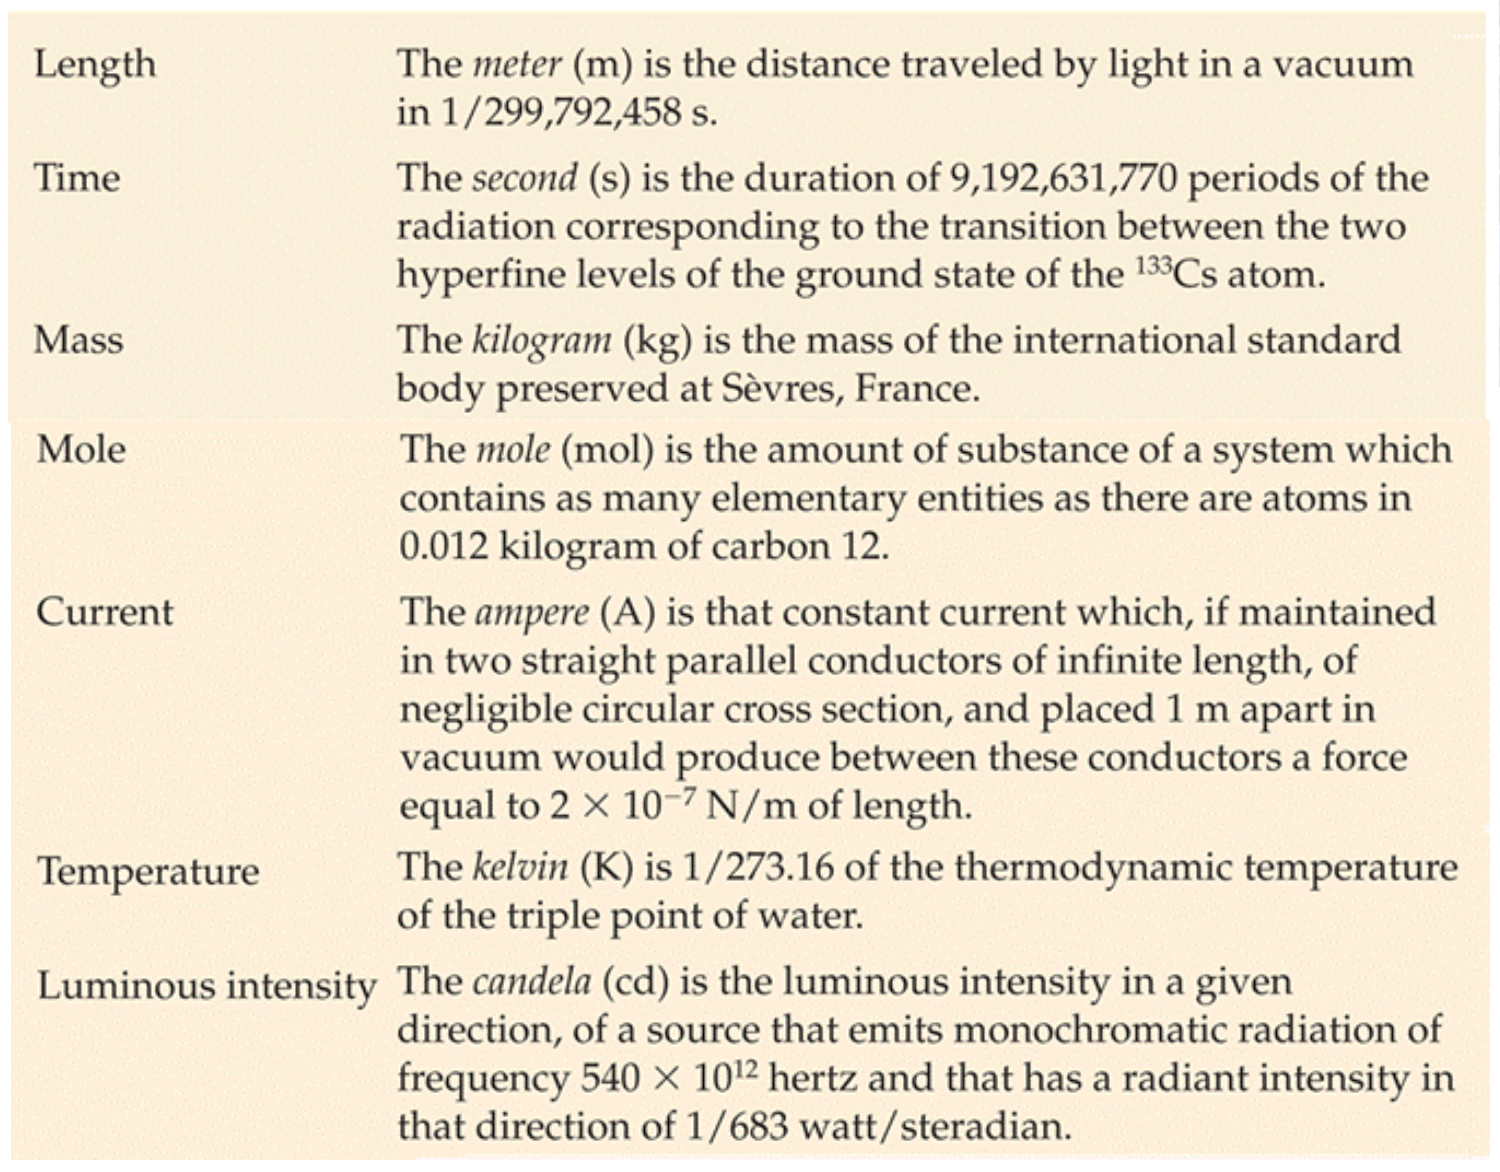
\includegraphics[width=1\textwidth]{imagenes/apendices/app01.png}
\end{figure}
\section{Notación científica. Múltiplos y submúltiplos}
\vspace{-5mm}\begin{figure}[H]
		\centering
		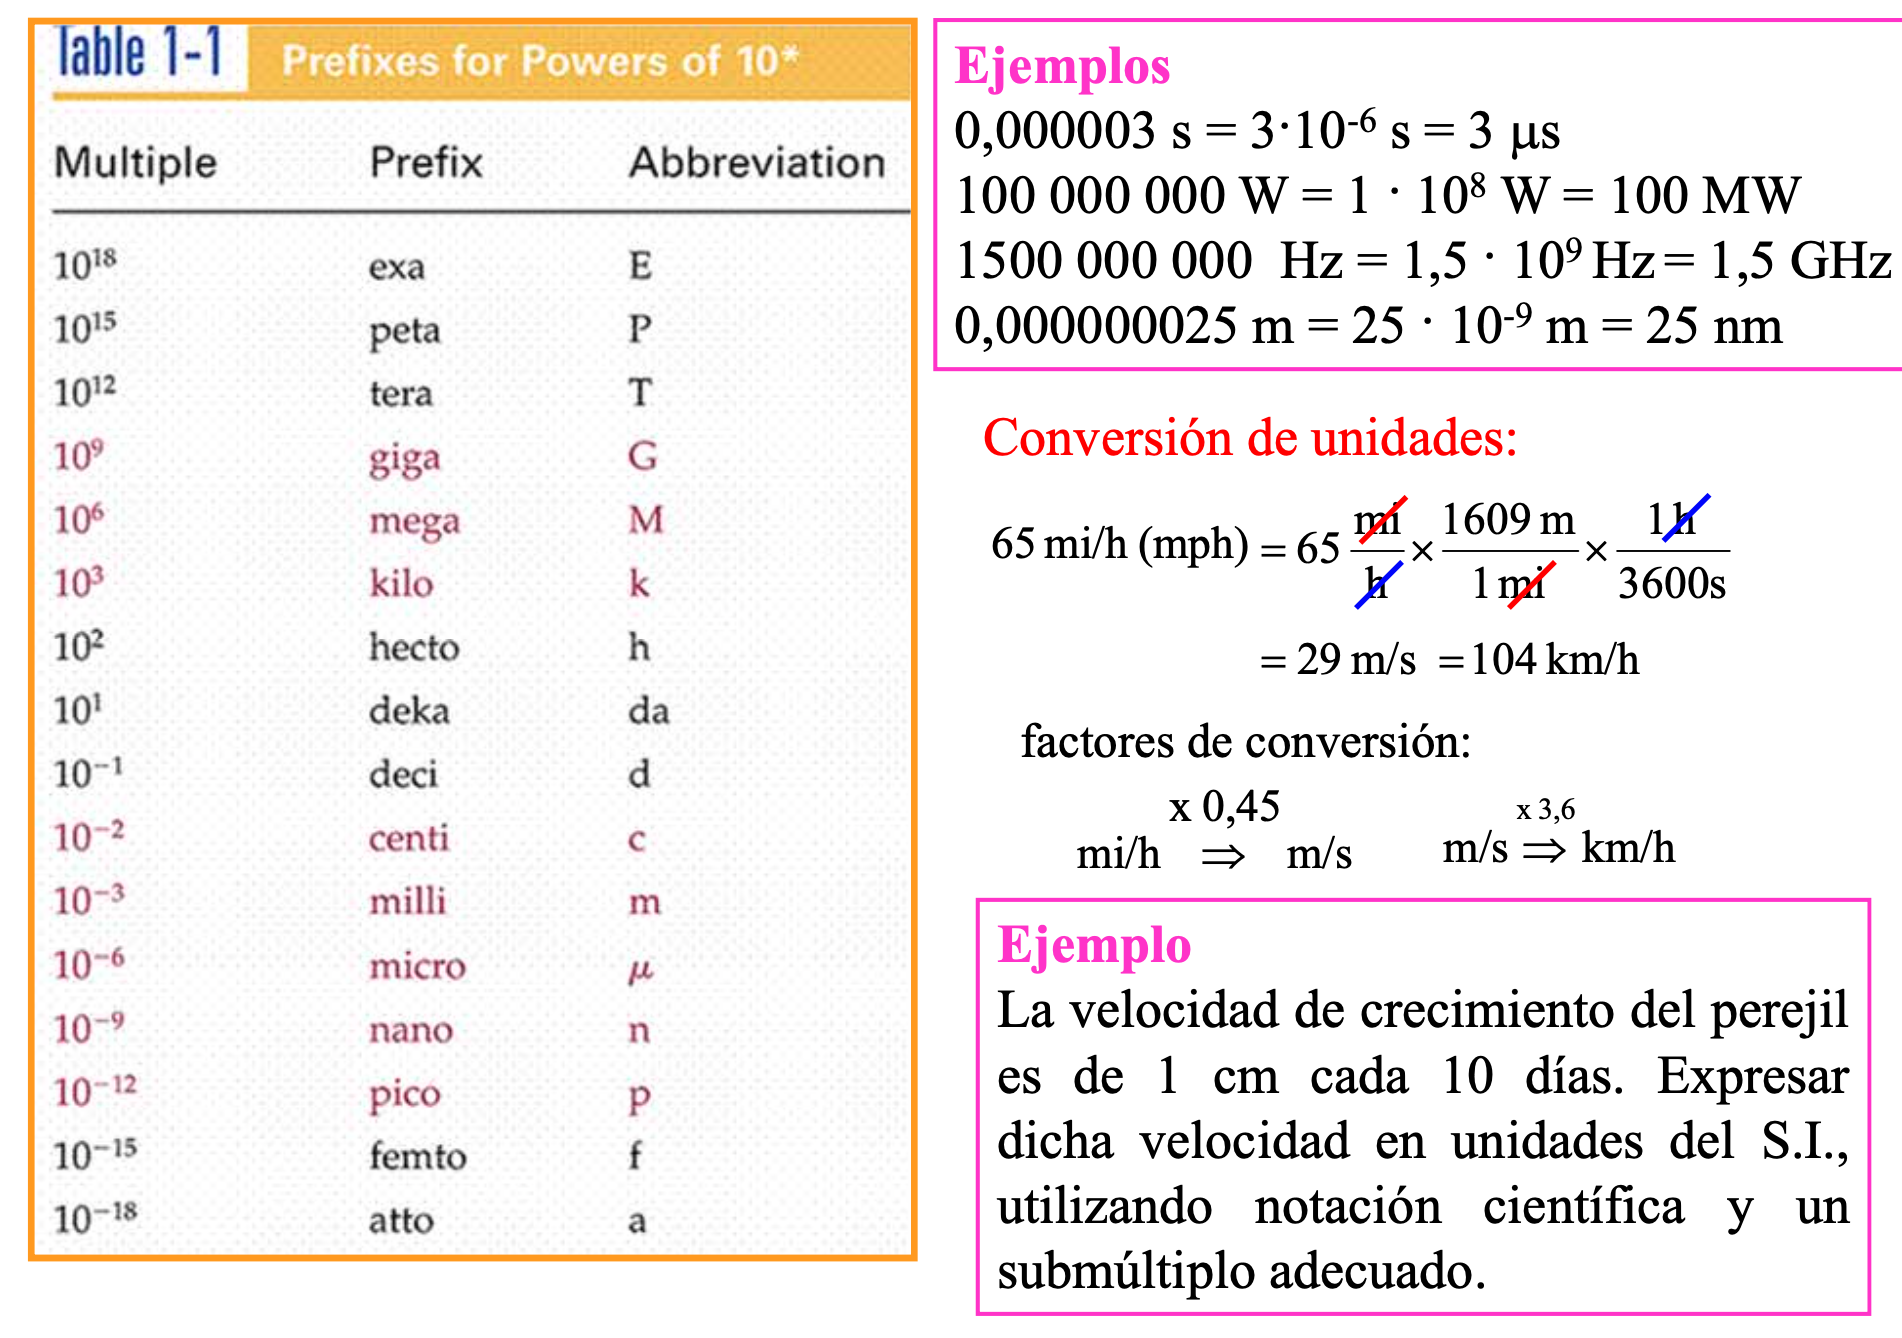
\includegraphics[width=.9\textwidth]{imagenes/apendices/app02.png}
\end{figure}
%\newpage
\vspace{-5mm}\section{Dimensiones y análisis dimensional}
\vspace{-5mm}\begin{figure}[H]
		\centering
		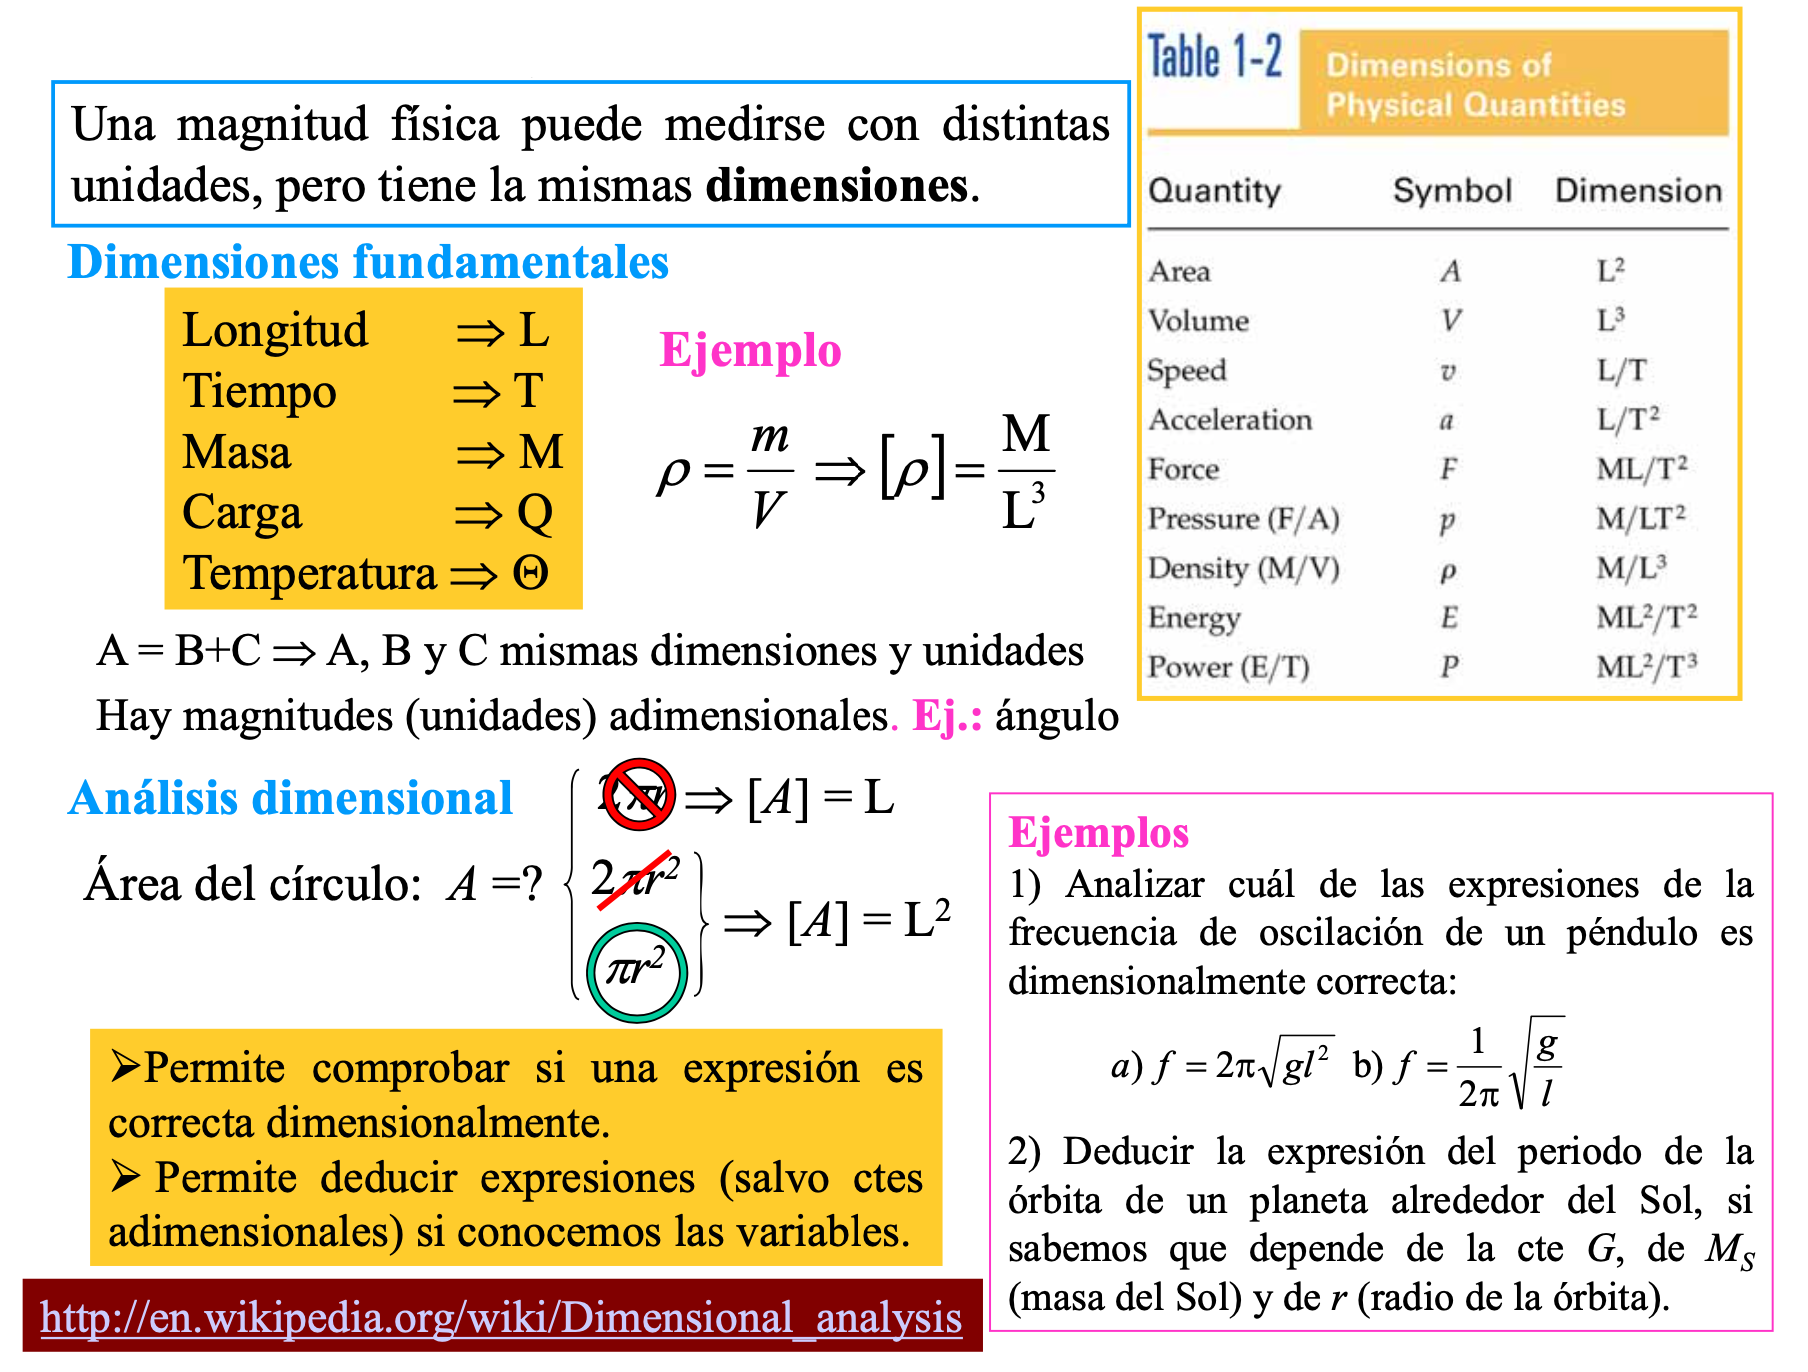
\includegraphics[width=.9\textwidth]{imagenes/apendices/app03.png}
\end{figure}
\vspace{-5mm}\section{Cifras significativas y órdenes de magnitud}
\vspace{-5mm}\begin{figure}[H]
		\centering
		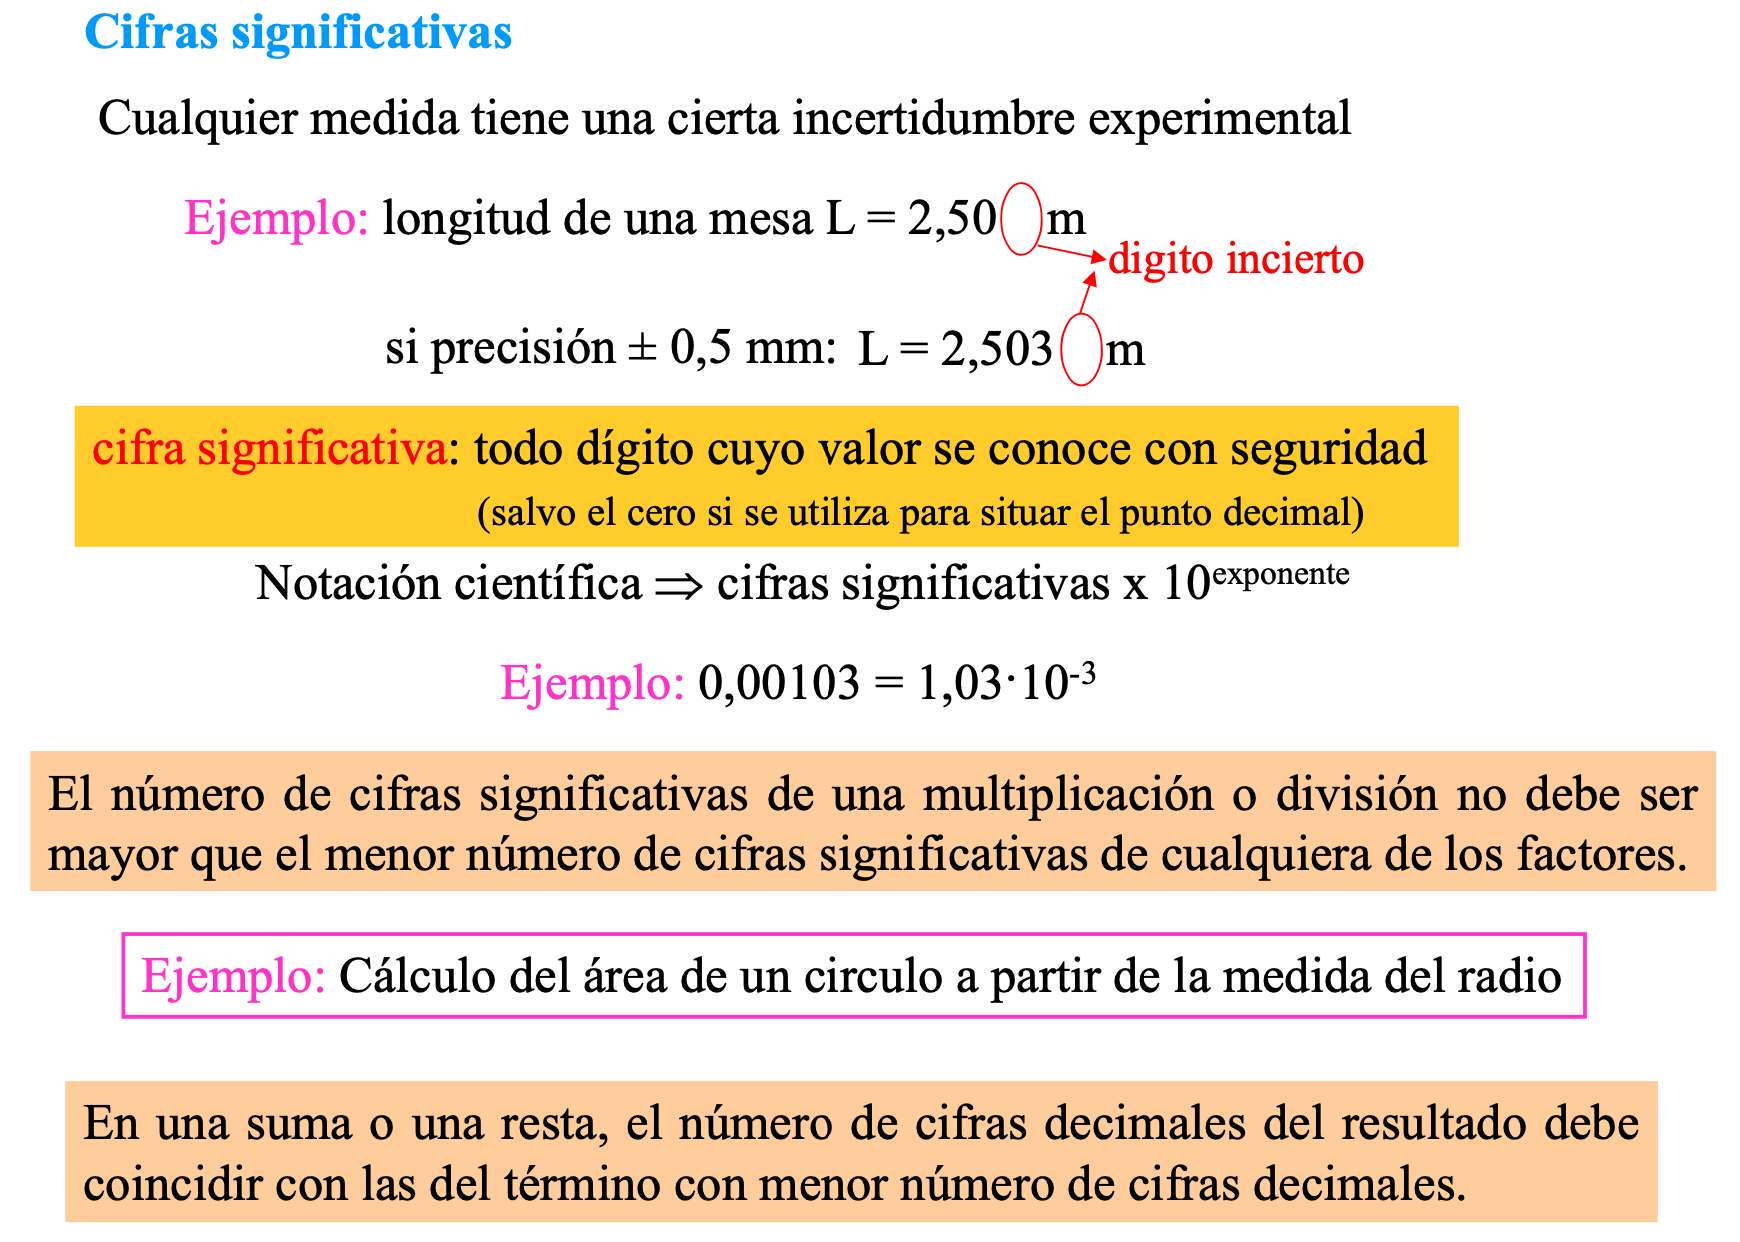
\includegraphics[width=.9\textwidth]{imagenes/apendices/app04.png}
\end{figure}
\vspace{-5mm}\begin{figure}[H]
		\centering
		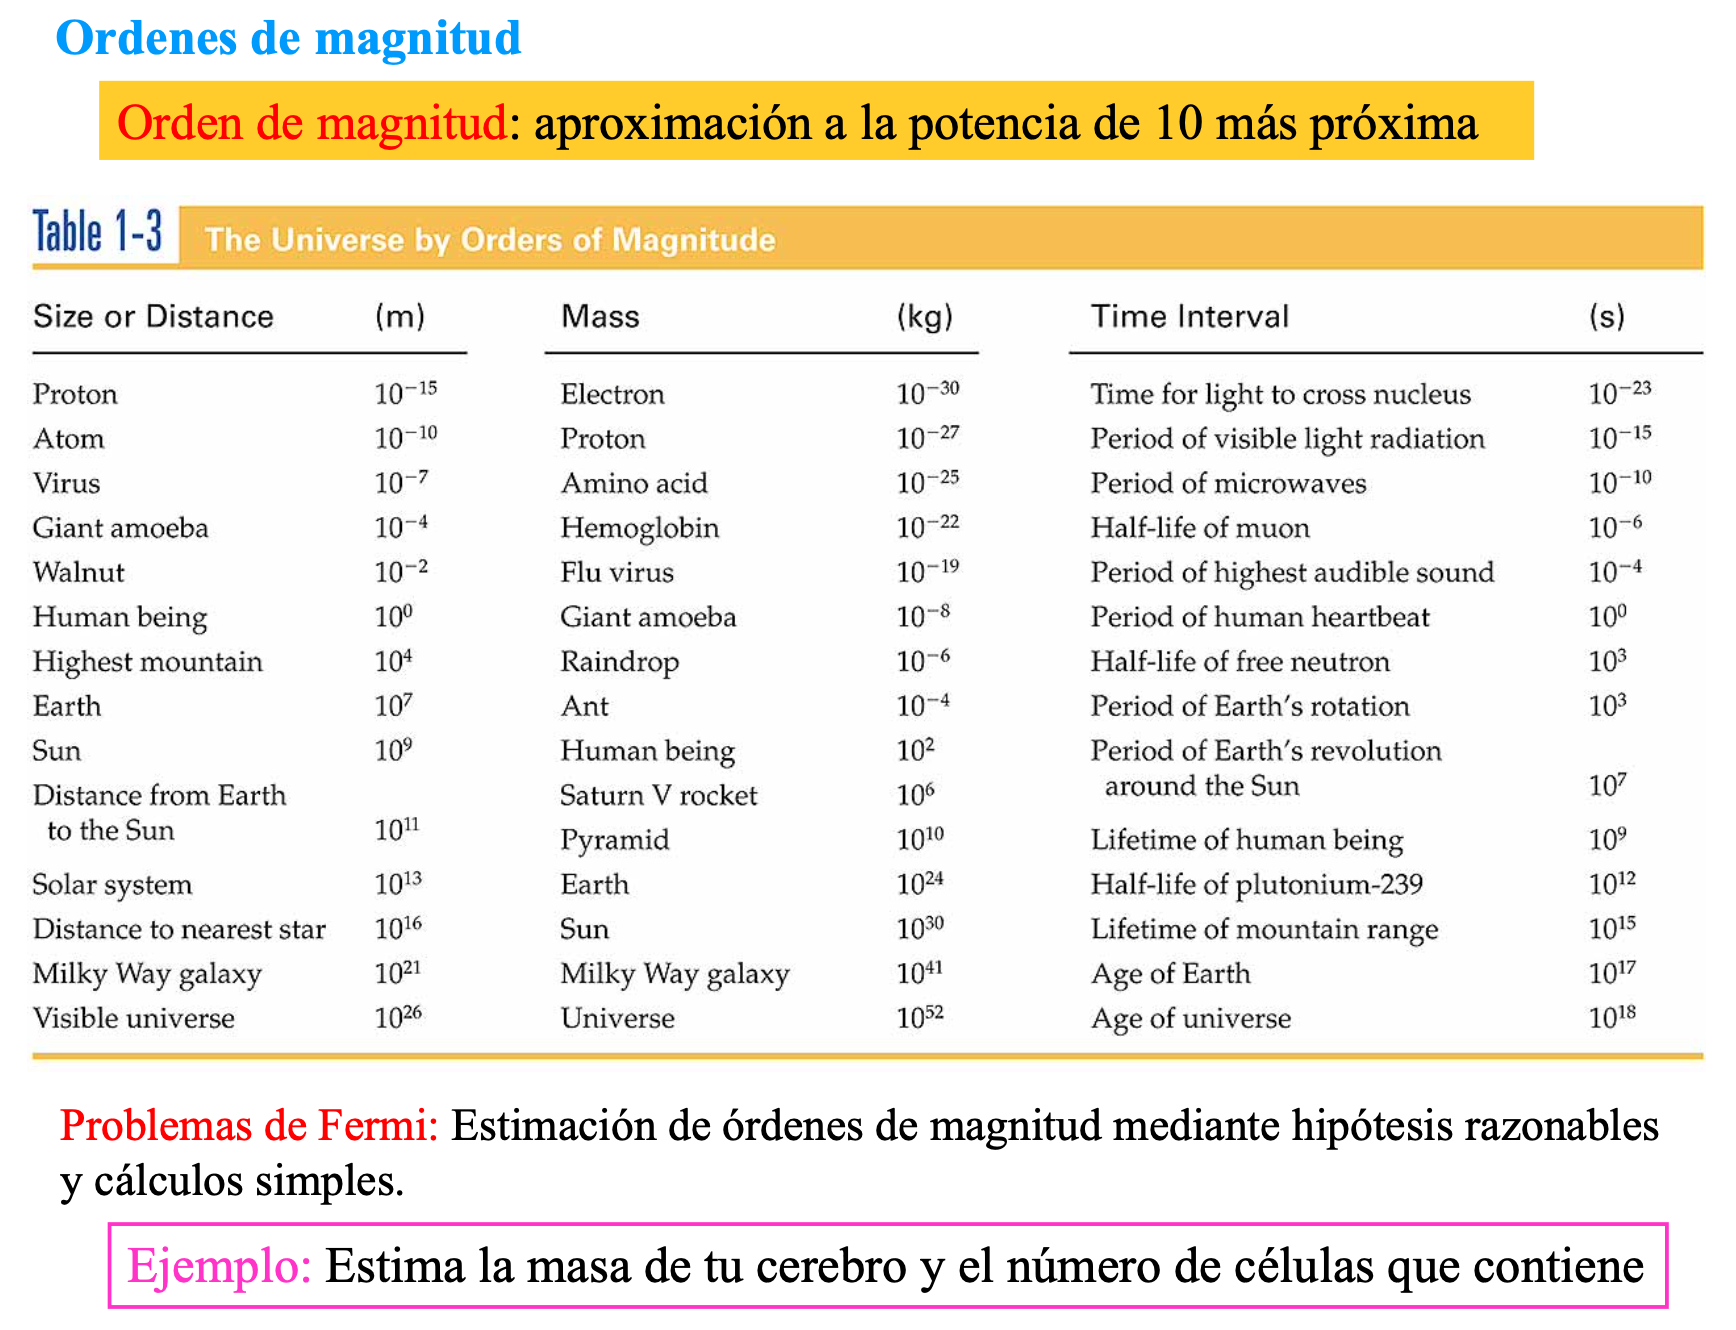
\includegraphics[width=.9\textwidth]{imagenes/apendices/app05.png}
\end{figure}


\chapter{Matemáticas preliminares para un curso de física general}
\chaptermark{Matemáticas preliminares}

\textsf{Se supone que quien desea seguir un curso de física general (nivel primero de carrera de la facultad de física), al acabar el bachillerato, domina el cálculo en una variable y es capaz de derivar e integrar con soltura. También es necesario que conozca y domine el concepto de vector libre y sus operaciones: producto escalar y vectorial; así como a operar con soltura en trigonometría y con números complejos.}

\textsf{Además de ello, conviene conocer los conceptos que desarrollamos someramente a continuación:} 
\vspace{-1mm} \begin{itemize}
\vspace{-1mm} \item \textsf{Desarrollos en serie de Taylor y Mclaurin.}
\vspace{-1mm} \item \textsf{Complejos. Fórmula de Euler: funciones trigonométricas e hiperbólicas.}
\vspace{-1mm} \item \textsf{Valor medio de una función.}	
\end{itemize}


\section{Desarrollos de Taylor y McLaurin} \label{McLaurin}

$f(x)$ función continua.

$I=\displaystyle \int_{x_0}^{x_0+h}f'(x) \dd x= \eval{f(x)}_{x_0}^{x_0+h}=f(x_0+h)-f(x_0) \qquad (1*)$

Cambio de variable: $t \; / \quad  x=x_0+h-t;\; \dd x= -\dd t$

$x_0 \text{ y } h$ son constantes, su derivada es cero.

$I=
\left[ \begin{matrix} x=x_0 & \to & h=t \\ x=x_0+h & \to & t=0  \end{matrix} \right]
=\displaystyle - \int_h^0 f'(x_o+h-t) \dd t=+\int_0^h f'(x_0+h-t) \dd t$

Integramos por partes

$I=\displaystyle \eval{f'(x_0+h-t)\cdot t}_0^h + \int_0^h f''(x_0+h-t) \dd t$

$I=\displaystyle f'(x_0)\ h+ \int_0^h f''(x_0+h-t)\ t \ \dd t$

Volvemos a integrar por partes

$I=\displaystyle f'(x_0)\ h+ \eval{f''(x_0+h-t)\ \dfrac {t^2}{2}}_0^h+\int_0^h \dfrac {t^2}{2}\ f'''(x_0+h-t) \ \dd t$

$I=\displaystyle f'(x_0)\ h + f''(x_0)\ \dfrac {h^2}{2!}+\int_0^h \dfrac {h^2}{2!}\ f'''(x_0+h-t)\ \dd t \quad (2*)$


Intuimos ya la ley de formación:

$I=\displaystyle f'(x_0) \ h +f''(x_0) \ \dfrac {h^2}{2!} + f'''(x_0) \ \dfrac {h^3}{3!}+ \cdots + f^{n)}(x)\ \dfrac {h^n}{n!}$

\textcolor{gris}{Notación: $\displaystyle f^{n)}(x_0)=\eval{\dv[n]{}{x} f(x)}_{x=x_0}$}

De (1*) y (2*), obtenemos el \textbf{desarrollo en serie de Taylor}

$\displaystyle \boxed{ \;\boldsymbol{ f(x_0+h)=f(x_0)+ f'(x_0) \ h +f''(x_0) \ \dfrac {h^2}{2!} + f'''(x_0) \ \dfrac {h^3}{3!}+ \cdots }\; }$

\textcolor{gris}{Hemos conseguido, para un punto $x_o+h$ próximo a $x_0$ sustituir la, en principio complicada, función $f(x)$ por un desarrollo en serie de potencias de $x$ (un polinomio), muchos más sencillo para el cálculo.}


Haciendo $x_0=0$ y $x=h$ obtenemos el \textbf{desarrollo es serie de McLaurin}

$\displaystyle \boxed{ \;\boldsymbol{ f(x)=f(0)+ f'(0) \ x +f''(0) \ \dfrac {x^2}{2!} + f'''(0) \ \dfrac {x^3}{3!}+ \cdots }\; }$


\textbf{Ejemplos} de funciones desarrolladas en serie de McLaurin son:

\begin{itemize}
\item \colorbox{LightYellow}{$\boldsymbol{e^x=1+x+}\displaystyle \dfrac {x^2}{2!}+\dfrac {x^3}{3!}+\dfrac {x^4}{4!}+ \cdots + \dfrac {x^n}{n!}+\cdots$}
\item \colorbox{LightYellow}{$\boldsymbol{\cos x= \displaystyle 1-\dfrac {x^2}{2!}}+\dfrac {x^4}{4!}-\dfrac {x^6}{6!}+ \cdots	$}
\item \colorbox{LightYellow}{$\boldsymbol{\sin x=\displaystyle x}-\displaystyle \dfrac {x^3}{3!}+\dfrac {x^5}{5!}\cdots $}	
\item \colorbox{LightYellow}{$\boldsymbol{\sqrt{1+x}=1+\dfrac 1 2 x}-\dfrac 1 8 x^2 +\dfrac 1 {16}x^3-\dfrac 5 {128}x^4 + \cdots $}	
\item \colorbox{LightYellow}{$\boldsymbol{\ln(x)?x-\dfrac{x^2}{2}+\dfrac{x^3}{3}+\cdots}$}	
\item \colorbox{LightYellow}{$\boldsymbol{\tan x=x+\dfrac 1 3 x^3+\dfrac 2 {15}x^3+\cdots}$}	
\item \colorbox{LightYellow}{$\boldsymbol{(1+x)^n=1+nx+\dfrac{n(n-1)}{2!}x^2+\dfrac{n(n-1)(n-2)}{3!}x^3+\cdots}$}		
\end{itemize}

Aplicación: $e^{-x^2}=1-x^2+\dfrac {x^4}{2!}-\dfrac {x^6}{3!}+\dfrac {x^8}{4!}+\cdots$

\begin{miparrafodestacado}
Para $x<<1$ son válidas las siguientes aproximaciones.

$\qquad (1+x)^n \approx 1+nx \ $ aproximación del binomio	

$\qquad e^x\approx 1 + x; \qquad \ln(1+x)\approx x$

$\qquad \sin x \approx x; \qquad \cos x\approx 1;\qquad \tan x\approx x$
\end{miparrafodestacado}


\section{Complejos}

$i=\sqrt{-1} \to z=x+i \ y; \quad x=\Re z;\;\; y=\Im z; \quad |z|=\sqrt{a^2+b^2}; \;\; \theta=\arctan \frac b a$


complejo conjugado: $z^*=x-i\ y;\qquad Z^2=z\ z^*$

$i^0=1;\quad i^1=i;\quad i^2=-1;\quad I^3=-i;\quad i^4=1;\quad \cdots$

Representación geométrica de $\mathcal C$. Diagrama de Argand.

\begin{multicols}{2}
$z\ = \ x+i\ y\ = \ r_{_\theta}$

$\quad$

$\left.
 \begin{matrix} x=r \cos \theta \\ y= r \sin \theta \end{matrix}
\quad  \right. \left| \quad 
\begin{matrix} r=\sqrt{x^2+y^2} \\ \tan \theta =\dfrac b a  \end{matrix} 
\right.$
\begin{figure}[H]
\centering
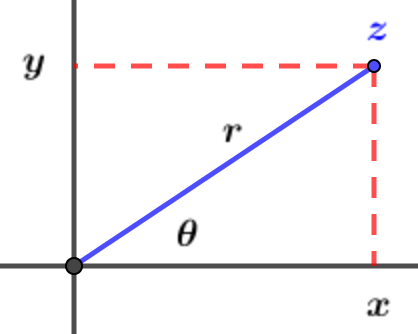
\includegraphics[width=0.30\textwidth]{imagenes/apendices/app06.png}
\end{figure}
\end{multicols}


Producto y cociente de complejos en forma polar:

$z_1\cdot z_2={(r_1\cdot r_2)}_{\ \theta_1+\theta_2} \qquad \dfrac {z_1}{z_2}={\left( \dfrac {r_1}{r_2} \right)}_{\ \theta_1+\theta_2}$

Fórmula de Moivre: $z^n=r^n\ (\cos n \theta + i\ \sin n\theta)$

\subsection{Funciones Trigonométricas}


$e^x=1+x+\displaystyle \dfrac {x^2}{2!}+\dfrac {x^3}{3!}+\dfrac {x^4}{4!}+ \cdots\quad$, sustituyendo $x$ por $i\theta$:


$e^{i\theta}=1+i\theta+ \dfrac {(i\theta)^2}{2!}+\dfrac {(i\theta)^3}{3!}+\dfrac {(i\theta)^4}{4!}+\cdots$

$e^{i\theta}=1+i\theta- \dfrac {\theta^2}{2!}-\dfrac {i\theta^3}{3!}+\dfrac {\theta^4}{4!}+\cdots $


Agrupando partes reales y partes imaginarias

$e^{i\theta}=
\left( 
1- \dfrac {\theta^2}{2!}+\dfrac {\theta^4}{4!}-\dfrac{\theta^6}{6!}+ \cdots
 \right) +
i\ \left( 
\theta-\dfrac {\theta^3}{3!}+\dfrac{\theta^5}{5!}-\dfrac{\theta^7}{7!}+\cdots
  \right) $

Identificando, la parte real es el desarrollo en serie del $\cos \theta)$ y la parte imaginaria del $\sin \theta$.

Luego: $\qquad$
\colorbox{LightYellow}{$\boxed{ \; \boldsymbol{ e^{i\theta}=cos \theta + i \ \sin \theta } \; } \qquad \qquad \text{\textbf{Fórmula de EULER}}$}

En general, $z=r\ (cos \theta + i \sin \theta) = r\ e^{i\theta}$

Es fácil comprobar que $e^{-i\theta}=\cos \theta - i\ \sin \theta$

Combinando estas expresiones:

\colorbox{LightYellow}{$\boxed{ \; \boldsymbol{ 
\cos \theta = \dfrac {e^{i\theta}+e^{-i\theta}}{2} \qquad \sin \theta=\dfrac{e^{i\theta}-e^{-i\theta}}{2i}
 } \; } $}

\subsection{Funciones Hiperbólicas}

Sustituimos $\theta$ po $z=x+i\ y$ en las dos fórmulas anteriores deducidas de la fórmula de Euler

$\cos z=\dfrac{e^{x+i\ y}+e^{-i\ (x+i\ y)}}{2}$

Operando: $\cos z=\dfrac{e^y+e^{-y}}{2} \ \cos x - i\ \dfrac{e^y-e^{-y}}{2} \ \sin x$ 

\emph{Por definición}, llamamos coseno y seno hiperbólicos a los coeficientes de $\cos x$ y $\sin x$ de la expresión anterior.

\colorbox{LightYellow}{$\boxed{ \; \boldsymbol{ 
\cosh y=\dfrac {e^y+e^{-y}}{2} \qquad \sinh y=\dfrac {e^y-e^{-y}}{2} 
 } \; } $}

$\cos z = \cosh y \ \cos x - i \ \sinh y \ \sin x; \qquad 
 \sin z = \cosh y \ \sin x + i \ \sinh y \ \cos x$
 
 Haciendo $x=0 \to z=0+i \ y \to \ \boldsymbol{\cos(iy)=\cosh y;\  \ \sin(iy)=\sin h y}$

Análogamente, $\quad \boldsymbol{\sinh (iy)=i\ \sin y; \qquad \cosh(iy)=\cos y}$

Es fácil demostrar que: $\displaystyle \quad \boldsymbol{\dv{\sinh y}{y}=\cosh y\; \qquad \dv{\cosh y}{y}=\sinh y}$

\vspace{20mm} %*********************************************
\section{Valor medio de una función}

\begin{multicols}{2}
El valor medio de una serie discreta es:

$\overline{x}=\dfrac{x_1+x_2+x_3+\cdots+x_N}{N}$

Tenemos dos magnitudes $x$ e $y$ relacionadas, $y=f(x)$, y hacemos $N$ observaciones.

$\text{si } \Delta x<<1 \to \text{ área }= y_i\cdot \Delta x$
\begin{figure}[H]
\centering
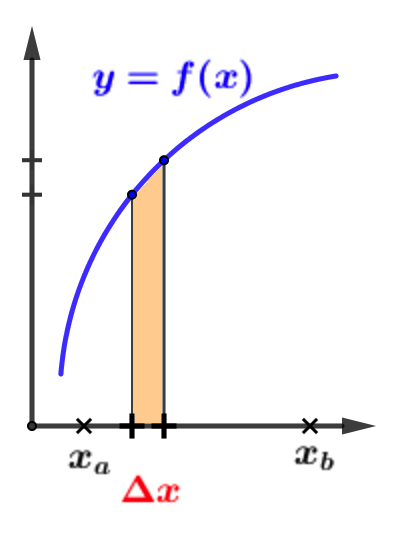
\includegraphics[width=0.30\textwidth]{imagenes/apendices/app07.png}
\end{figure}	
\end{multicols}


El área total

$S=\displaystyle \sum_{i=1}^{N}(y_i\ \Delta x_i)=\sum_{i=1}^{N}(y_i)\ \Delta x=N \ \overline{y} \ \Delta x=\overline{y}\ (x_b-x_a)$, por lo que

$\overline{y}=\displaystyle \dfrac 1{x_b-x_a} \ \sum_{i=1}^N y_i\ \Delta x$

Para una función continua, tomando límites con $\Delta x\to 0$

\colorbox{LightYellow}{$\boxed{ \; \boldsymbol{ 
\overline{y}=<y>=\displaystyle \dfrac 1{x_b-x_a} \ \int_{x_a}^{x_b}f(x) \ \dd x = \dfrac 1{x_b-x_a} \ \int_{x_a}^{x_b} y \  \dd x
 } \; } $}




\chapter{Vectores}\label{Vectores}

\section{Vectores en el espacio ($\mathbb R^3$)}


$\vec v= \overrightarrow { AB }  $: segmento orientado. Origen A y extremo B
	\begin{multicols}{2}		
	\begin{itemize}
	\item \textit{módulo}: $|\vec v|=d(A,B)$
	\item \textit{dirección}: la de la recta $r$ y la de todas las paralelas a $r$
	\item \textit{sentido}: desde $A$ hacia $B$
	\end{itemize}
	\begin{figure}[H]
		\centering
		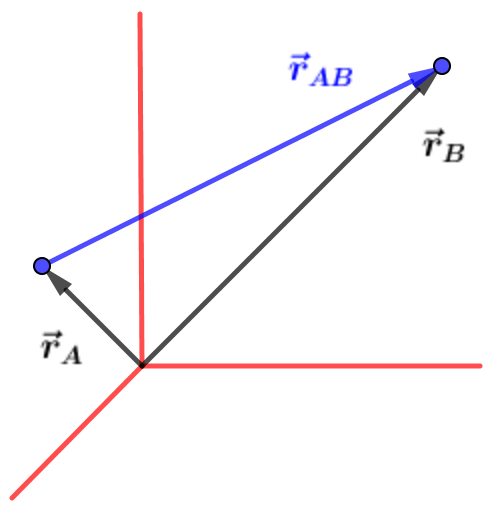
\includegraphics[width=0.3\textwidth]{imagenes/apendices/T10IM01.png}
	\end{figure}
	\end{multicols}

Vectores LIBRES, se pueden trasladar paralelamente a sí mismos por todo el espacio.
				
Dos vectores son IGUALES si tienen el mismo módulo, la misma dirección y el mismo sentido.

\section{Producto de un vector por un escalar}

$k \in \mathbb{R}; (\text{escalar})$: $\ \ k\cdot \vec v$
\begin{multicols}{2}				
\begin{itemize}
	\item \textit{módulo}: $|k|\cdot |\vec v|$
	\vspace{-2mm}\item \textit{dirección}: la misma que $\vec v$
	\vspace{-2mm}\item \textit{sentido}: si $k>0$ mismo que $\vec v$; si $k<0$ contrario a $\vec v$
\end{itemize} 
\begin{figure}[H]
		\centering
		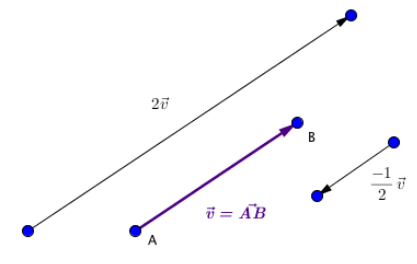
\includegraphics[width=0.25\textwidth]{imagenes/apendices/T10IM02.png}
\end{figure}
\end{multicols}


Dado un vector $\vec v$, un vector UNITARIO en la misma dirección que $\vec v$ se puede obtener como: $\dfrac 1 {|\vec v|}\cdot \vec v$

\vspace{4mm}

\underline{Propiedades:} 

\begin{itemize}
\begin{multicols}{2}
	\item $a\cdot (b\cdot \vec v)=(a\cdot b)\cdot \vec v$ 
	\item  $a\cdot (b\cdot \vec v)=(a\cdot b)\cdot \vec v$ 
	\item $(a+b)\cdot \vec v=a\cdot \vec v+ b\cdot \vec v  $
	\item $1\cdot \vec v=\vec v$
\end{multicols}
\end{itemize}

\section{Suma de vectores}

	$\vec u \pm \vec v$  (gráficamente: en matemáticas se usa la técnica de vectores concurrentes, en física es más usual el método del paralelogramo).
	\begin{multicols}{2}
	
	\begin{itemize}
		\item $(\vec u + \vec v)+ \vec w=\vec u+(\vec v + \vec w)$
		\vspace{-2mm}\item $\vec u + \vec v= \vec v+ \vec u$
		\vspace{-2mm}\item $\vec u+ \vec 0=\vec u$
		\vspace{-2mm}\item $\vec u+ (\overrightarrow {-u})=\vec 0$
	\end{itemize}
	\begin{figure}[H]
		\centering
		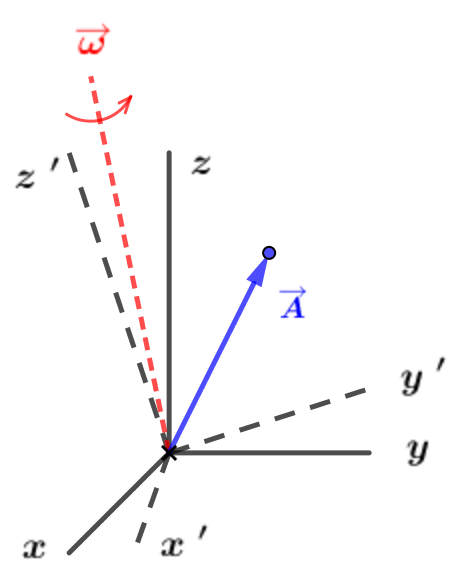
\includegraphics[width=0.5\textwidth]{imagenes/apendices/T10IM03.png}
	\end{figure}
	\end{multicols}
	Restar vectores = sumar el opuesto : $\vec u - \vec v = \vec u +(-\vec v)$

\begin{multicols}{2}
	\scriptsize{Puesto que los vectores con que tratamos son libres, el `método del paralelogramo' usado en física consiste en colocar los vectores unidos por sus orígenes y, mediante paralelas a éstos, construir un paralelogramo. El vector que va desde la unión de los vectores al punto opuesto de la diagonal es el vector suma}  \normalsize{:}

	\begin{figure}[H]
	\centering
	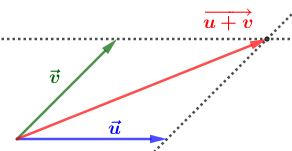
\includegraphics[width=0.3\textwidth]{imagenes/apendices/T10IM14.png}
	\end{figure}
\end{multicols}

\begin{multicols}{2}
	\begin{figure}[H]
	\centering
	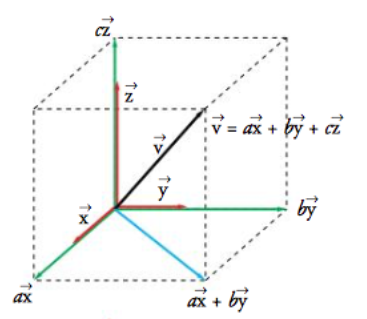
\includegraphics[width=0.25\textwidth]{imagenes/apendices/T10IM04.png}
	\end{figure}
	
	La suma de tres vectores de distinta dirección y no coplanarios en el espacio: 
	
	\centerline{$\vec u+\vec v+\vec w$} 
	
	es la diagonal del paralelepípedo.
\end{multicols}

\vspace{-5mm} \section{Combinación lineal de vectores}

	Dados varios vectores $\vec u_1$, $\vec u_2$, $\vec u_3$, ..., $\vec u_n$ y otros tantos números reales $\alpha_1$, $\alpha_2$, $\alpha_3$, ..., $\alpha_n$, a la expresión $\alpha_1 \vec u_1+\alpha_2 \vec u_2+\alpha_3 \vec u_3+...+\alpha_n \vec u_n$ se le llama `Combinación Lineal' de los n-vectores iniciales.
		
	%\vspace{3mm}
		
	Varios vectores se dice que son `Linealmente Dependientes'  si alguno de ellos se puede poner como combinación lineal de los demás. Si no es así, se dice que son `Linealmente Independientes'.
	

\section{Base}

\begin{multicols}{2}
	3 vectores cualesquiera del espacio, no coplanarios, y de direcciones distintas, $\vec x,\ \vec y, \ \vec z$ son linealmente independientes, además, cualquier otro vector del espacio se puede escribir como combinación lineal de estos tres vectores de forma única. Se dice que estos tres vectores forman una BASE $B=\{\vec x,\ \vec y, \ \vec z\}$
	\begin{figure}[H]
	\centering
	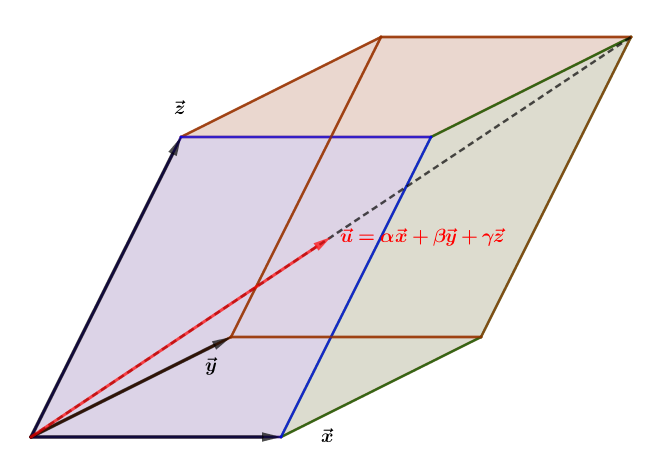
\includegraphics[width=0.4\textwidth]{imagenes/apendices/T10IM06.png}
	\end{figure}
\end{multicols}

\vspace{30mm} %**********************************************

\begin{multicols}{2}
	\begin{figure}[H]
	\centering
	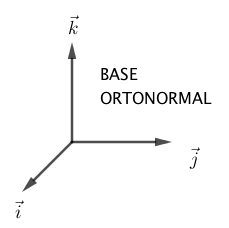
\includegraphics[width=0.25\textwidth]{imagenes/apendices/T10IM05.png}
	\end{figure}
	Si los vectores de la base son mutuamente perpendiculares (ortonormales) y tienen módulo 1 (unitarios), la base $B=\{\vec i, \vec j, \vec k \}$ se llama `Base OrtoNormal (BON)' 
	\footnotesize{(Orto por ortogonal, es decir, perpendiculares entre sí, y Normal porque los vectores básicos tiene norma o módulo $1$, están normalizados)}\normalsize{.}
\end{multicols}

\section{Operaciones en componentes}

Como cualquier vector $\vec v$  se puede expresar de forma única en cada base $B=\{\vec x,\ \vec y, \ \vec z\} \quad \to \quad \vec v= \alpha \vec x+ \beta \vec y+ \gamma \vec z$. A los parámetros de esta combinación lineal, $\alpha, \ \beta, \ \gamma$ se les llama \underline{componentes} de $\vec v$ en la base $B$, $\ \vec v=(\alpha, \ \beta, \ \gamma)$
		
Las componentes de $\vec i, \ \vec j, \ \vec k$ en la base ortonormal $B=\{ \vec i, \vec j, \vec k \} $ son $\vec i=(1,0,0); \ \vec j=(0,1,0); \ \vec k=(0,0,1)$
		
 En el espacio, los \underline{puntos} se representan por \underline{coordenadas}, $A(x_0, y_0, z_0)$ y los \underline{vectores} por \underline{componentes} $\vec u=(u_x, u_y, u_z)$


		
\vspace{3mm} $ \alpha , \ \beta \ \in \mathbb{R}; \ \vec u=(u_x,u_y,u_z); \ \vec v = (v_x ,v_y ,v_z) \to $
		
\vspace{2mm}\hspace{20mm}$\alpha \vec u+\beta \vec v=
			(\alpha  u_x+\beta  v_x,\;  \alpha  u_y+\beta  v_y,\;  \alpha  u_z+\beta  v_z) $
			
\section{Producto `Escalar'}

\begin{equation}
	\boxed{\ \vec u \cdot \vec v = |\vec u| \cdot |\vec v| \cdot \cos \theta \ } \ ,\ \in \mathbb{R} 
\end{equation}			

\vspace{30mm} %**********************************************
\begin{multicols}{2}
Geométricamente:

\emph{El producto escalar de dos vectores es el módulo de uno de ellos por la proyección del otro sobre él}
\begin{figure}[H]
	\centering
	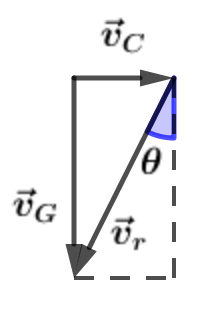
\includegraphics[width=0.25\textwidth]{imagenes/apendices/T10IM07.png}
\end{figure}
\end{multicols}


	Propiedad fundamental: $\forall \  \vec u,\ \vec v\ \neq 0:\ \boxed{\  \vec u \bot \vec v \ \leftrightarrow \ \vec u \cdot \vec v=0 \ }$
		
	$\vec u \cdot \vec v = \vec v \cdot \vec u$; $\ \alpha ( \vec u \cdot \vec v) =( \alpha \vec u) \cdot \vec v = \vec u \cdot ( \alpha \vec v)$; $\ \vec u \cdot (\vec v + \vec w)= \vec u \cdot \vec v + \vec u \cdot \vec w$
		
	 Módulo de un vector: $\boxed{ \ | \vec u |=+\sqrt{\vec u \cdot \vec u} \ }$
		
	 Ángulo entre dos vectores: $\boxed{ \ \cos \theta = \dfrac {\vec u \cdot \vec v}{|\vec u| \cdot |\vec v|} \ }$
	 
\vspace{4mm} \textbf{Producto escalar en B.O.N. \small{(Base orto-normal)}}

$BON=\{ \vec i, \vec j, \vec k \ / \  |\vec i|=|\vec j|=|\vec k|=1 \ \wedge \ \vec i \bot \vec j; \ \vec j \bot \vec k; \ \vec k \bot \vec i \}$. 

$\vec u=(u_1,u_2,u_3); \ \vec v=(v_1, v_2, v_3) \ \to \ $
$\boxed{   \vec u \cdot \vec v= u_1 v_1+u_2 v_2+u_3 v_3  }  \ \in \mathbb{R}$

\vspace{2mm} Módulo en una BON: $ \vec u=(u_1,u_2,u_3) \to |\vec u|=+\sqrt{u_1^2+u_2^2+u_3^2}$
		
\vspace{2mm} Ángulo \small{de dos vectores en una BON:} $\cos \theta = \dfrac {u_1 v_1+u_2 v_2+u_3 v_3}{\sqrt{u_1^2+u_2^2+u_3^2}\cdot \sqrt{v_1^2+v_2^2+v_3^2}}$

\vspace{4mm}

\begin{multicols}{2}
\textit{Normalización de un vector:} 

Dado un vector $\vec v$, conseguir otro de la misma dirección pero de módulo $1$, le llamaremos $\vec u_v$ y se obtiene como: $\vec u_v=\dfrac {1}{|\vec v|}\cdot \vec v = (\cos \alpha, \cos \beta, \cos \gamma)$, son los llamados \textit{cosenos directores} (las componentes de todo vector unitario).
\begin{figure}[H]
	\centering
	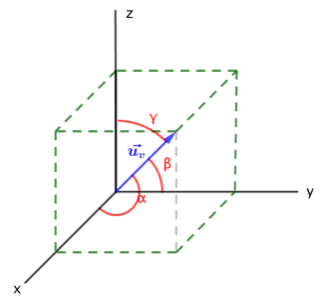
\includegraphics[width=0.30\textwidth]{imagenes/apendices/T10IM08.png}
\end{figure}
\end{multicols}

\section{Producto `Vectorial'}

El producto vectorial de dos vectores $\vec u$ y $\vec v$ es un nuevo vector $\vec u \times \vec v$	 tal que:
\begin{multicols}{2}
\begin{itemize}
\item su módulo es $|\vec u \times \vec v|=|\vec u||\vec v| \sin \theta $, siendo $\theta$ el ángulo que forman $\vec u$ y $\vec v$.
\item su dirección es perpendicular al plano que forman $\vec u$ y $\vec v$.
\item y su sentido es el del giro de un `sacacorchos' que intente llevar el vector$\vec u$ hacia el $\vec v$.
\end{itemize}
\begin{figure}[H]
	\centering
	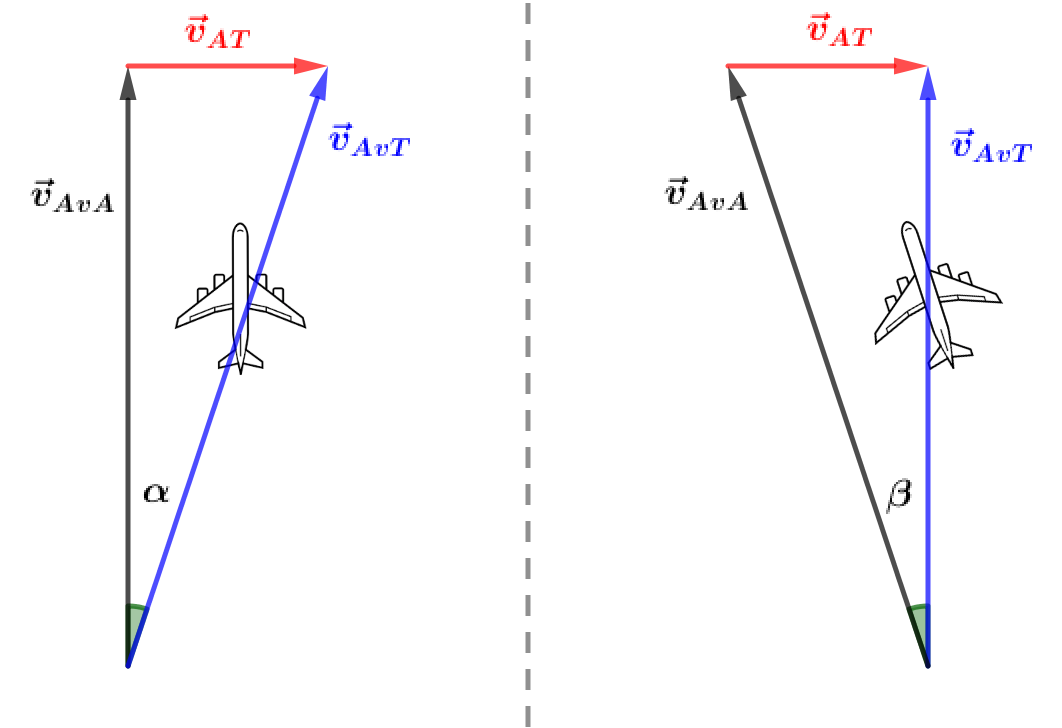
\includegraphics[width=0.30\textwidth]{imagenes/apendices/T10IM09.png}
\end{figure}
\end{multicols}

\textbf{Propiedades del producto vectorial.}
\begin{multicols}{2}

El \underline{módulo} del producto vectorial mide el \underline{área del paralelogramo} que forman los vectores $\vec u$ y $\vec v$.
				
\hspace{10mm}$|\vec u \times \vec v|=|\vec u||\vec v| \sin \theta$

\begin{figure}[H]
	\centering
	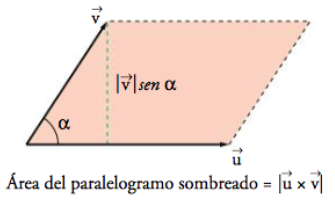
\includegraphics[width=0.30\textwidth]{imagenes/apendices/T10IM10.png}
\end{figure}

\end{multicols}

\begin{itemize}
	\item ¡El producto vectorial es \underline{no-conmutativo}!: $\vec u \times \vec v=-\vec v \times \vec u$
	\item $\vec u \times \vec u=\vec 0$
	\item Tomaremos la BON \underline{orientada}, $\vec i \times \vec j = \vec k$; $\vec j \times \vec k = \vec i$ y $\vec k \times \vec i = \vec j$

A esto es lo que llaman los físicos una BON `orientada', los vectores $\vec i, \vec j, \vec k$ no pueden tener orientaciones cualesquiera. 	

\item $(\alpha \vec u)\times \vec v=\alpha (\vec u \times \vec v)= \vec u \times (\alpha \vec v)$
\item ¡\underline{No} se cumple la \underline{asociativa}!: $\vec u \times (\vec v \times \vec w) \neq (\vec u \times \vec v)\times \vec w$
\item \underline{Distributivas}: $\vec u \times (\vec v + \vec w)= \vec u \times \vec v + \vec u \times \vec w$; $(\vec u + \vec v)\times \vec w=\vec u \times \vec w + \vec v \times \vec w$
\item En componentes, el desarrollo del producto vectorial es un determinante:
\begin{equation}		
\boxed{ \ \overrightarrow { u } \times \overrightarrow { v } \quad =\quad \left| \begin{matrix} \overrightarrow { i }  & \overrightarrow { j }  & \overrightarrow { k }  \\ u_1 & u_2 & u_3 \\ v_1 & v_2 & v_3 \end{matrix} \right| \ }
\end{equation}
\end{itemize}
		
\vspace{2mm}$\vec u \times \vec v$ siempre es un vector perpendicular a $\vec u$ y a $\vec v$ y su módulo representa el área del paralelogramos que defines estos dos vectores.

\vspace{5mm} ¡ Afortunadamente, el producto vectorial no es asociativo XD !

\begin{figure}[H]
	\centering
	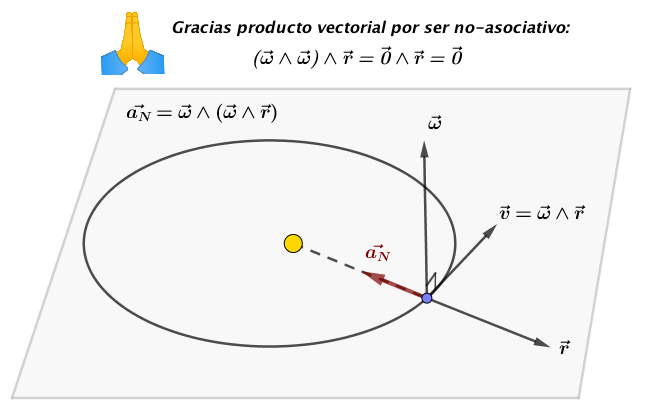
\includegraphics[width=1\textwidth]{imagenes/apendices/T10IM11.png}
\end{figure}

\section{Producto `Mixto'}
\begin{equation}
\boxed{ \ [\vec u, \vec v, \vec w]=\vec u \cdot (\vec v \times \vec w)=|\vec u|\cdot|(\vec v \times \vec w)|\cdot \cos \theta \ }
\end{equation}

\begin{multicols}{2}
El \underline{producto mixto} $[\vec u, \vec v, \vec w]$ mide, \underline{en valor absoluto}, el \underline{volumen del paralelepípedo} formado por los tres vectores.
				
En componentes se calcula como un determinante:
				
$\boxed{ \ [\overrightarrow { u } ,\overrightarrow { v }, \overrightarrow { w }]  \quad =\quad \left| \begin{matrix} u_{ 1 } & u_{ 2 } & u_{ 3 } \\ v_{ 1 } & v_{ 2 } & v_{ 3 } \\ w_{ 1 } & w_{ 2 } & w_{ 3 } \end{matrix} \right| \ } $

\begin{figure}[H]
	\centering
	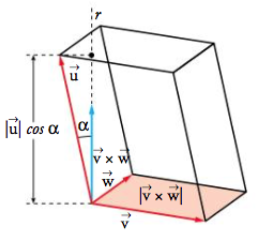
\includegraphics[width=0.35\textwidth]{imagenes/apendices/T10IM12.png}
\end{figure}
\end{multicols}

\begin{multicols}{2}
Por propiedades de los determinantes y del valor absoluto podemos afirmar que para el cálculo del volumen de un paralelepípedo formado por tres vectores no importa el orden en que los cojamos para calcular el producto mixto.
\begin{figure}[H]
	\centering
	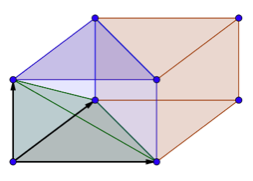
\includegraphics[width=0.20\textwidth]{imagenes/apendices/T10IM13.png}
\end{figure}
\end{multicols}


\section{Ejercicios resueltos}


\begin{ejre}
	Obtén 3 vectores perpendiculares a $\vec u=(3,2,7)$, no proporcionales entre sí
\end{ejre}

\begin{proof}\renewcommand{\qedsymbol}{$\diamond$}.
	
	\begin{multicols}{2}
	Sabemos que  
	$  \vec u \bot \vec v \ \leftrightarrow \ \vec u \cdot \vec v=0 \ $
	y que vectores perpendiculares a uno dado hay infinitos (todo un `plano vectorial'), y que cualquier combinación de dos vectores perpendiculares a uno dado también es perpendicular a éste.
	\begin{figure}[H]
	\centering
	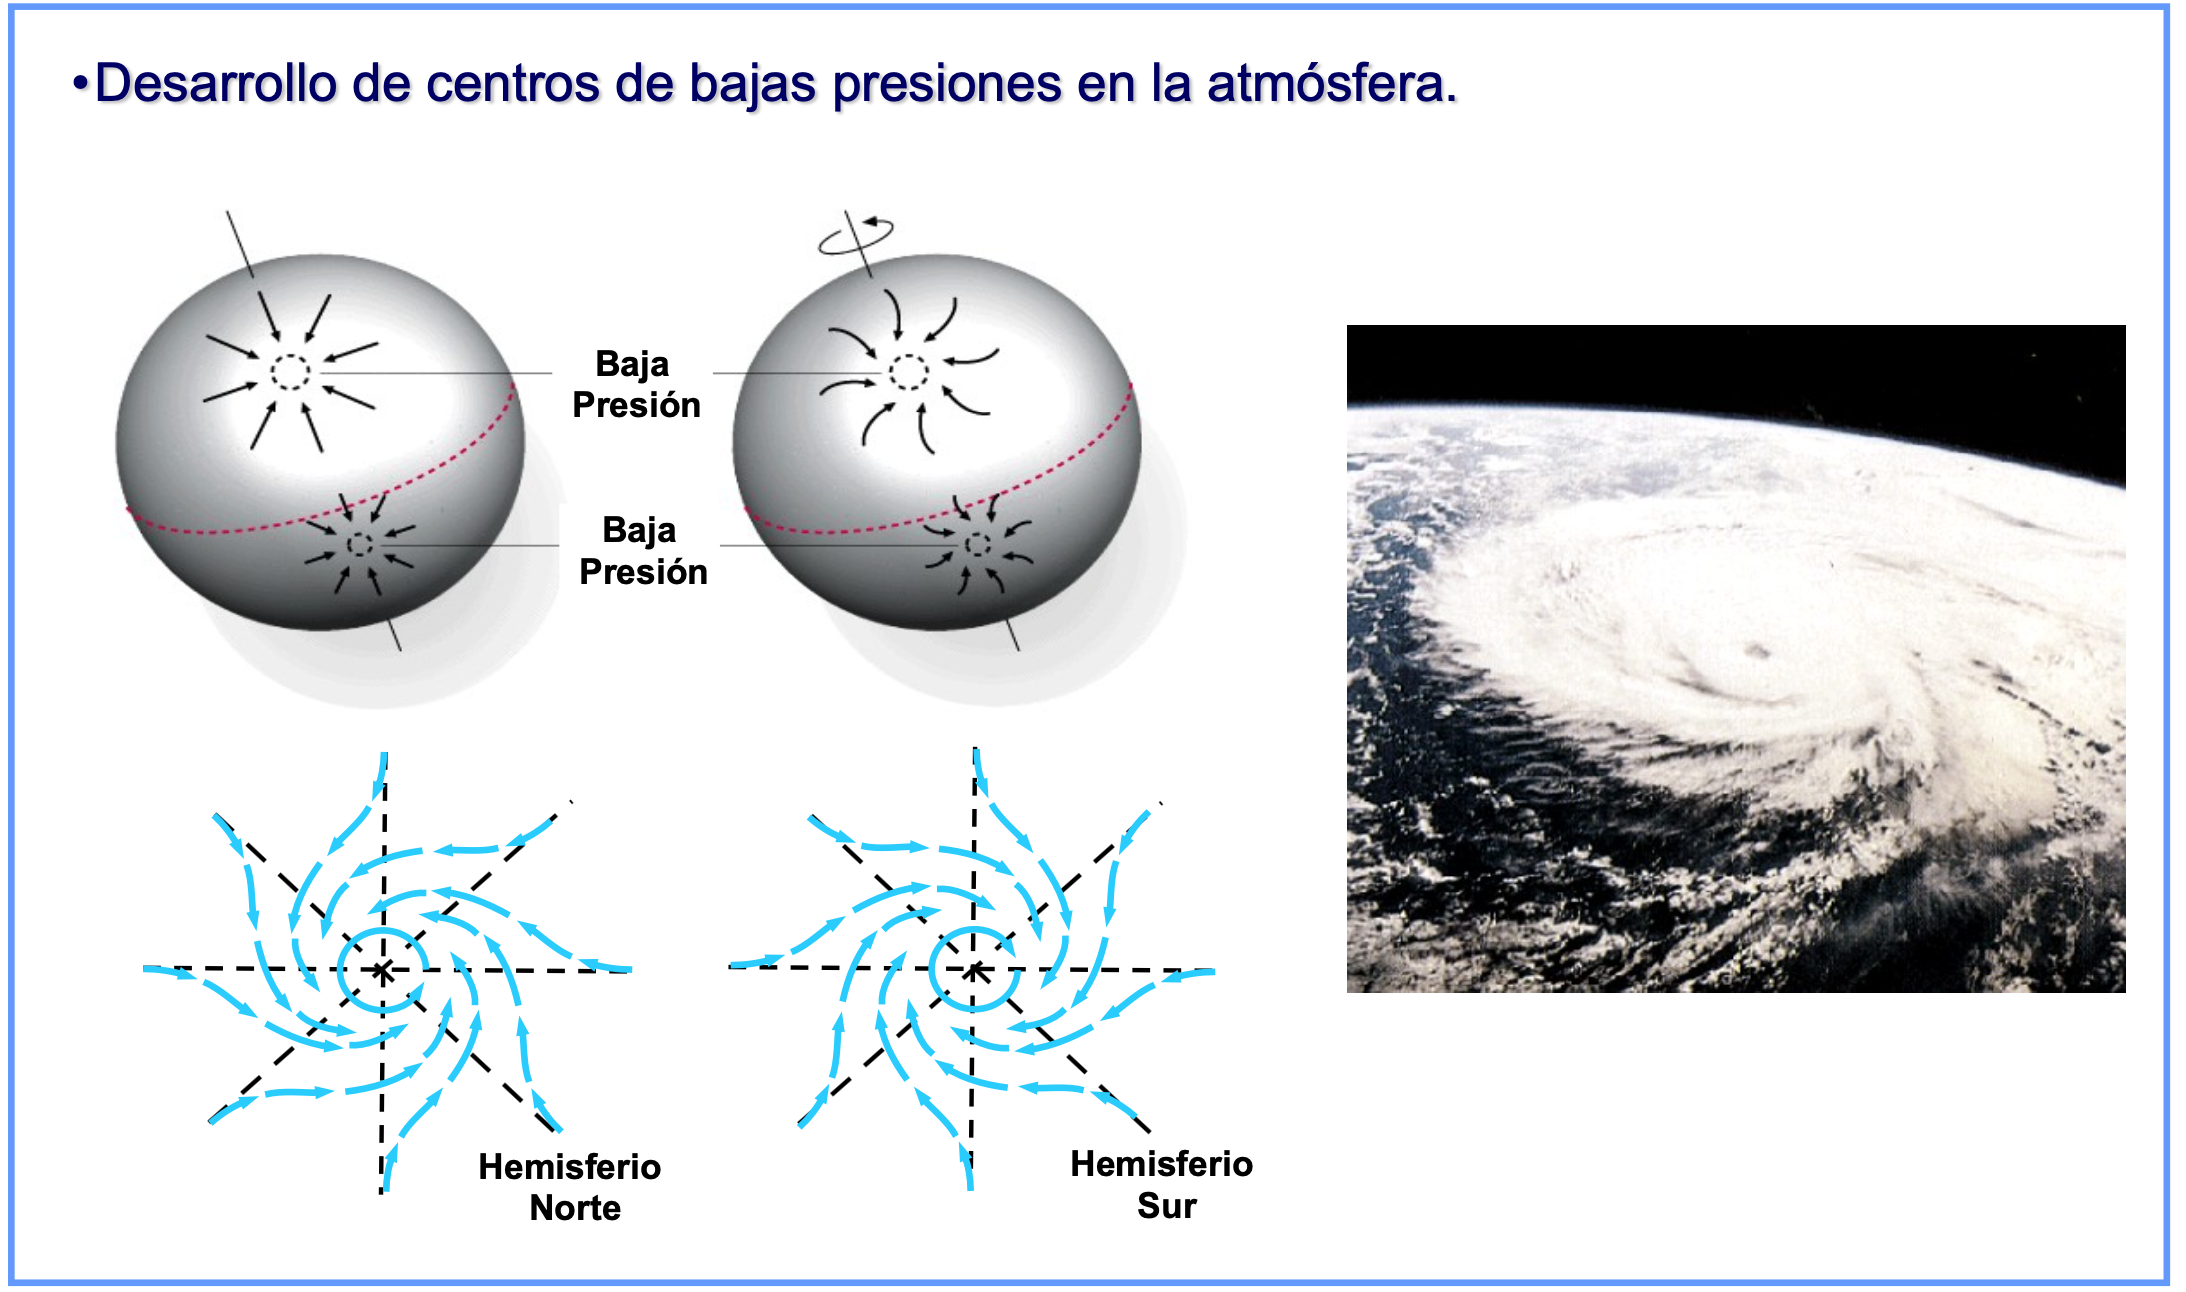
\includegraphics[width=0.30\textwidth]{imagenes/apendices/T10IM15.png}
	\end{figure}	
	\end{multicols}	
	Solo tenemos que encontrar vectores $\vec {v_i}$ tales que $\vec u \cdot \vec {v_i}=0$. Por ejemplo:
	
	$\vec {v_1} = (0,-7,2) \to \vec u \cdot \vec {v_1}=(3,2,7)\cdot (0,-7,2)=3 \cdot 0 + 2 \cdot (-7) + 7 \cdot 2 =-14+14=0$
	
	Compruébese que $\ \vec {v_2} = (7,0,-3);  \quad \vec {v_3} = (2,-3,0) \ $ también son perpendiculares a $\vec u$
	
	También es perpendicular a $\vec u$ cualquier combinación lineal de estos tres vectores encontrados, como p.e.:
	$\ \vec {v_4}  = \vec {v_2}+\vec {v_3}= (9,-3-3)$; incluso si lo simplificamos dividiendo por 3 (multiplicar un vector por $\frac 1 3 $  proporciona un vector de la misma dirección: $\vec {v'_4}=(3,-1,-1) \to   \ \vec u \bot \vec {v'_4} $ (\emph{compruébese}).
	
	Otro más: $\vec {v_5}=\vec {v_1} - 2 \vec {v_2}+ 3\vec {v_3}= (8,-18,8)$ (\emph{compruébese}).
\end{proof}


\begin{ejre}

	Dados:  $\vec u=(1,0,-1); \vec v=(2,3,1)$. Calcular $u \cdot v; |u|; |v|; \cos \theta $
\end{ejre}


\begin{proof}\renewcommand{\qedsymbol}{$\diamond$}
.

$u \cdot v = (1,0,-1) \cdot (2,3,1)=2+0-1=1$

$|\vec u|=+\sqrt{1^1+0^2+(-1)^2}=\sqrt{2}\; ; \quad |\vec v|=+\sqrt{2^2+3^2+1^2}=\sqrt{14}$

$\vec u \cdot \vec v = |\vec u|\cdot |\vec v| \cdot \cos \theta \to 
1=\sqrt 2 \, \sqrt{14} \; \cos \theta \to \cos \theta = \frac {\sqrt{7}}{14} \textcolor{gris}{\to \theta=79.1^o}  $

	
\end{proof}


\begin{ejre}
	Obtén un vector perpendicular a $\vec u=(3,-1,2)$ y  a $\vec v=(1,0,3)$.
\end{ejre}

\begin{proof}\renewcommand{\qedsymbol}{$\diamond$}
	
	Lo más sencillo es buscar el vector producto vectorial de ambos: $ \vec w =\vec u \times \vec v$
	
	$\overrightarrow { w } =\left| \begin{matrix} \vec { i }  & \vec { j }  & \vec { k }  \\ 3 & -1 & 2 \\ 1 & 0 & 3 \end{matrix} \right| =[\text{ Sarrus }] =-3\vec { i } -7\vec { j } +\vec { k } =(-3,-7,1)$
\end{proof}


\begin{ejre}
	Calcula el área del rectángulo de vértice  $A(2,3,7)$, $B(1,-5,4)$  y  $C(7,0,11)$
\end{ejre}

\begin{proof}\renewcommand{\qedsymbol}{$\diamond$}
	
	Con los vértices $A, B,$ y $C$, formamos los vectores $\vec u=\overrightarrow {AB}$ y $\vec v=\overrightarrow {AC}$. Por definición del producto vectorial, el área del triángulo será igual a $ \frac 1 2 \; | \vec u \times \vec v |$

$\vec u=\overrightarrow {AB}=B-A=(-1,-8,-3)$ y $\vec v=\overrightarrow {AC}= C-A=(5, -3, 4)$.

$\overrightarrow { u \times v } =\left| \begin{matrix} \vec { i }  & \vec { j }  & \vec { k }  \\ -1 & -8 & -3 \\ 5 & -3 & 4 \end{matrix} \right| ==-41\vec { i } -11\vec { j } +43\vec { k } =(-41,-11,43)$

$|\overrightarrow { u \times v } | = \sqrt{(-41)^2+(-11)^2+(43)^2}\approx 60.42$

Área triángulo $ \approx  \frac 1 2 \; 60.41 = 30.21\; u^2$

¡Atención!: si al calcular el área de un triángulo dado por sus tres vértices el resultado es cero $\to$ ' los tres puntos están alineados'.
\end{proof}

%5
\begin{ejre}
	Calcula el volumen del tetraedro cuyos vértices son: $A(-7,-2,5), B(0,2,0), C(-9,3,8)$  y $D(-7,5,9)$; 
\end{ejre}

\begin{proof}\renewcommand{\qedsymbol}{$\diamond$}

Formamos los vectores:

$\vec u = \overrightarrow {AB}=B-A=(7,4,-5)$; 
$\vec v = \overrightarrow {AC}=C-A=(-2,5,3)$; 
$\vec w = \overrightarrow {AD}=D-A=(0,7,4)$

Sabemos que el valor absoluto del producto mixto de estos tres vectores es el volumen del paralelepípedo que forman, que su mitad es el volumen del prima y la sexta parte la del tetraedro, que es lo que nos piden, así que: 

Volumen tetraedro = $\frac 1 6 \left|\;  \left[ vec\quad u,\quad vec\quad v,\quad vec\quad w \; \right] \right|  =\left| \;  \left| \begin{matrix} 7 & 0 & 3 \\ -2 & 5 & 3 \\ 0 & 7 & 4 \end{matrix} \right|\;  \right| =\frac 1 6 \; |95|= \frac {95}{6} \; u^2$	
\end{proof}


\begin{ejre}
	Calcula el volumen de paralelepípedo (y del prisma y del tetraedro) formado por los vectores libres $\vec u=(3,1,2), \vec v=(4,-1,0)\  y\  \vec w=(3,6,2)$
\end{ejre}

\begin{proof}\renewcommand{\qedsymbol}{$\diamond$}
	
	$\left[ vec\quad u,\quad vec\quad v,\quad vec\quad w \right] =\left| \begin{matrix} 3 & 1 & 2 \\ 4 & -1 & 0 \\ 3 & 6 & 2 \end{matrix} \right| =40$
	
	$Vol_{paral}  = 40 \;  u^3; \quad  Vol_{prism} = \frac {40}2 =20\; u^3; \quad Vol_{tetr} = \frac {40}6 = 20/3 \; u^3$
	
\end{proof}

\begin{ejre}
	Calcular él ángulo que forman dos diagonales de un cubo.
\end{ejre}

\begin{proof}\renewcommand{\qedsymbol}{$\diamond$}
\begin{multicols}{2}	
	\begin{figure}[H]
	\centering
	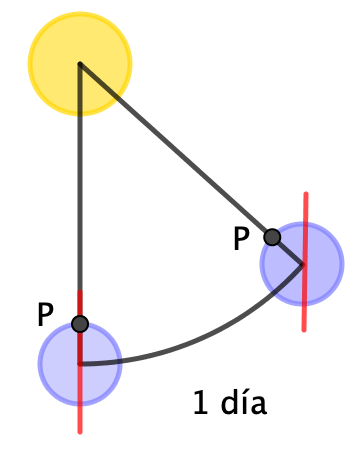
\includegraphics[width=0.30\textwidth]{imagenes/apendices/T10IM16.png}
	\end{figure}
De las 4 diagonales del cubo (no diagonales de las caras), elegimos las de la figura, con vectores asociados: $\overrightarrow{OD}=D-O=(l,l,l)-)0,0,0)=(1,1,1)\; l\; $ y $\overrightarrow{EC}=C-E=(0,0,l)-(l,l,0)=(1,-1,-1)\; l$

Calcule el lector el ángulo entre estos vectores con ayuda del producto escalar. \scriptsize{( $\theta \approx 109.5^0$, las diagonales, como rectas: $180-109.5=	70.5^0$)}

\end{multicols}
\end{proof}



\chapter{Vectores en diferentes sistemas de coordenadas}
\chaptermark{Vectores $\neq$ Sist. Coord.}
 \label{VectoresDistintosSistemasCoordenadas}

En coordenadas cartesianas o rectangulares, las componentes del vector de posición de un punto $P(x,y,z)$ son: $\boldsymbol{ \vec r}=\overrightarrow{\mathcal O P}=\boldsymbol{ x\vec i+y\vec j+ z \vec k}$

\section{Sistema de coordenadas cilíndricas}

La posición de un punto $P$ viene dado, en cilíndricas, por dos distancias y un ángulo $P(r,\theta,z)$ y los vectores unitarios son $\overrightarrow{u_r}$,  $\overrightarrow{u_{\theta}}$, $\vec k$.


El vector unitario $\vec k$ , se aplica en el punto $P$ y es paralelo al eje $OZ$.

El vector unitario $\overrightarrow{u_r}$ se aplica en $P$ y es paralelo al vector $\vec r$ dibujado en el plano $XY$, estando determinado por la proyección de $P$ sobre el citado plano.

El vector unitario $\overrightarrow{u_{\theta}}$ se aplica en $P$ y es perpendicular a los otros dos verificando $\vec k \times \overrightarrow{u_r}=\overrightarrow{u_{\theta}}$.

El vector de posición de un punto $P$ viene determinado por $\vec R=r \vec u_r+z\vec k$, no quedando unívocamente determinado.


\begin{figure}[H]
	\centering
	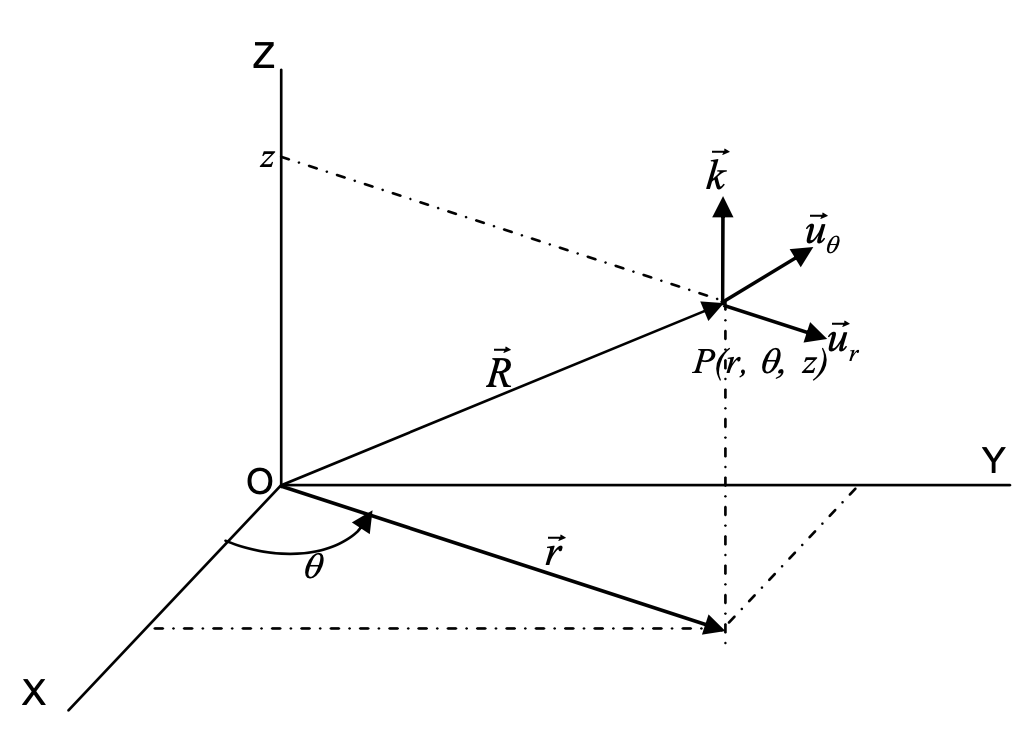
\includegraphics[width=.75\textwidth]{imagenes/apendices/APENDICESIM34.png}
\end{figure}


RELACIÓN DE LOS SISTEMAS DE COORDENADAS CILÍNDRICAS Y RECTANGULARES.

Buscamos las relaciones de $\overrightarrow{u_r}$, $\overrightarrow{u_{\theta}}$ con los vectores $\vec i$ y $\vec j$, pues $\vec k$ es el mismo en ambos sistemas de coordenadas. Para ello, trasladamos $\overrightarrow{u_r}$ y $\overrightarrow{u_{\theta}}$ al plano $XY$:

\begin{figure}[H]
	\centering
	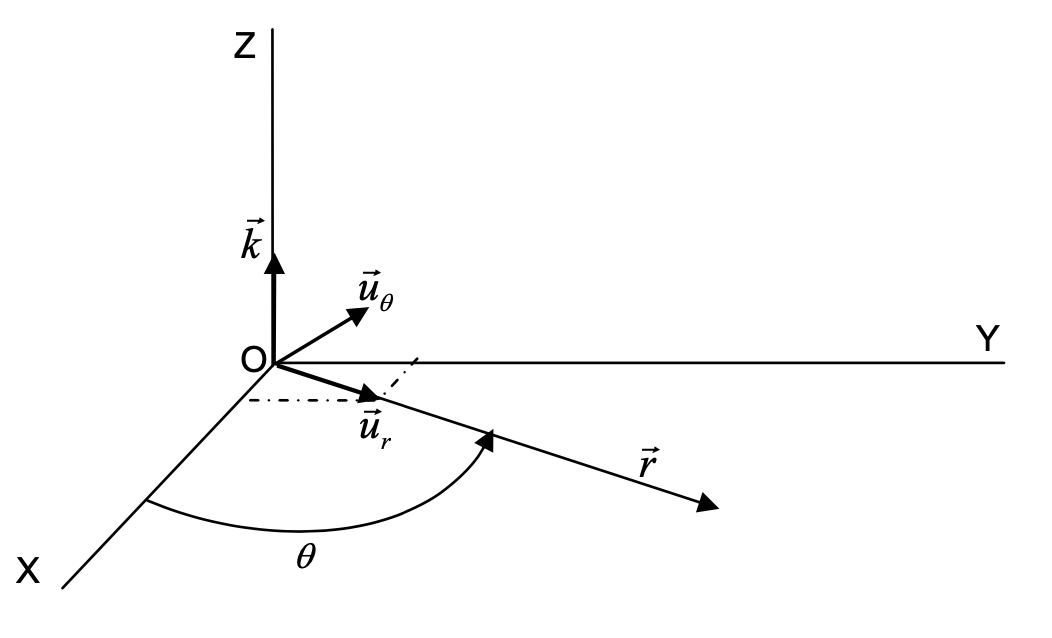
\includegraphics[width=.75\textwidth]{imagenes/apendices/APENDICESIM34b.png}
\end{figure}

Como $\overrightarrow{u_r}$ y $\overrightarrow{u_{\theta}}$  son unitarios $\to \abs{\overrightarrow{u_r}}=\abs{\overrightarrow{u_{\theta}}}=1$ 

$$ \overrightarrow{u_r}= \cos \theta \vec i + \sin \theta \vec j$$
$$ \overrightarrow{u_{\theta}}=\cos \left(\theta+\dfrac \pi 2 \right) \vec i + \sin \left(\theta+\dfrac \pi 2 \right) \vec j=-\sin \theta \vec i + \cos \theta \vec j$$
$$\vec k=\vec k$$

\begin{ejem}
	Un punto tiene por coordenadas cartesianas $P(4,3,2)$, ¿cuáles son sus coordenadas cilíndricas?
\end{ejem}
$\abs{\vec r}=\sqrt{4^2+3^2}=5 \quad \to \quad P_C=r\vec \;{u_r} + z \; \vec k = 5\; \vec {u_r}+2 \; \vec k$
\vspace{5mm}\begin{ejem}
Expresa el vector $\vec v=-8\vec i+10\vec j-12\vec k$ en coordenadas cilíndricas si su punto de aplicación está en $P(4,3,2$	
\end{ejem}
Calculemos primero los vectores unitarios $\overrightarrow{u_r}$, $\overrightarrow{u_{\theta}}$, $\vec k$ en el punto $P(4,3,2)$:


$\cos \theta=x/r=4/5=0.8; \quad \sin \theta=y/r=3/5=0.6$

$\overrightarrow{u_r} =\cos \theta \vec i + \sin \theta \vec j=0.8\vec i + 0.6 \vec j$, 

$\overrightarrow{u_{\theta}}=\-sin \theta \vec i + \cos \theta \vec j=-0.6\vec i + 0.8 \vec j$

\vspace{2mm}Para expresar $\vec v$ en cilíndricas, $\vec {v_C}$, hemos de calcular sus componentes en las direcciones de $\overrightarrow{u_r}$, $\overrightarrow{u_{\theta}}$y $\vec k$  que no es más que la proyección del vector sobre los vectores unitarios, que por serlo, coincide con el producto escalar ($\vec i$, $\vec j$, $\vec k$ forman una BON):

\vspace{2mm} $\vec v \cdot \vec {u_r}=(-8\vec i +10\vec j-12 \vec k)\cdot (0.8\vec i + 0.6 \vec j)=-6.4+6=-0.4$

$\vec v \cdot \vec {u_{\theta}}=(-8\vec i +10\vec j-12 \vec k)\cdot (-0.6\vec i + 0.8 \vec j)=4.8+8=12.8$

$\vec v \cdot \vec k=(-8\vec i +10\vec j-12 \vec k)\cdot (1\vec k)=-12$


Por lo que: $\quad \vec {a_C}=-0.4\; \vec {u_r}+12.8\; \vec {u_{\theta}}-12\; \vec k$

Compruébese que $\abs{\vec {v_c}}=\sqrt{308}=\abs{\vec v}$. El módulo es el mismo, obviamente, independientemente del sistema de coordenadas elegido.

\section{Sistema de coordenadas esféricas}
La posición de un punto $P$ queda determinado por una distancia $r$ y dos ángulos $\theta$ y $\phi$, $P(r,\theta,\phi)$.  Los vectores unitarios son $\vec u_{r}$ $\vec u_{\theta}$, $\vec u_{\phi}$.

\begin{figure}[H]
	\centering
	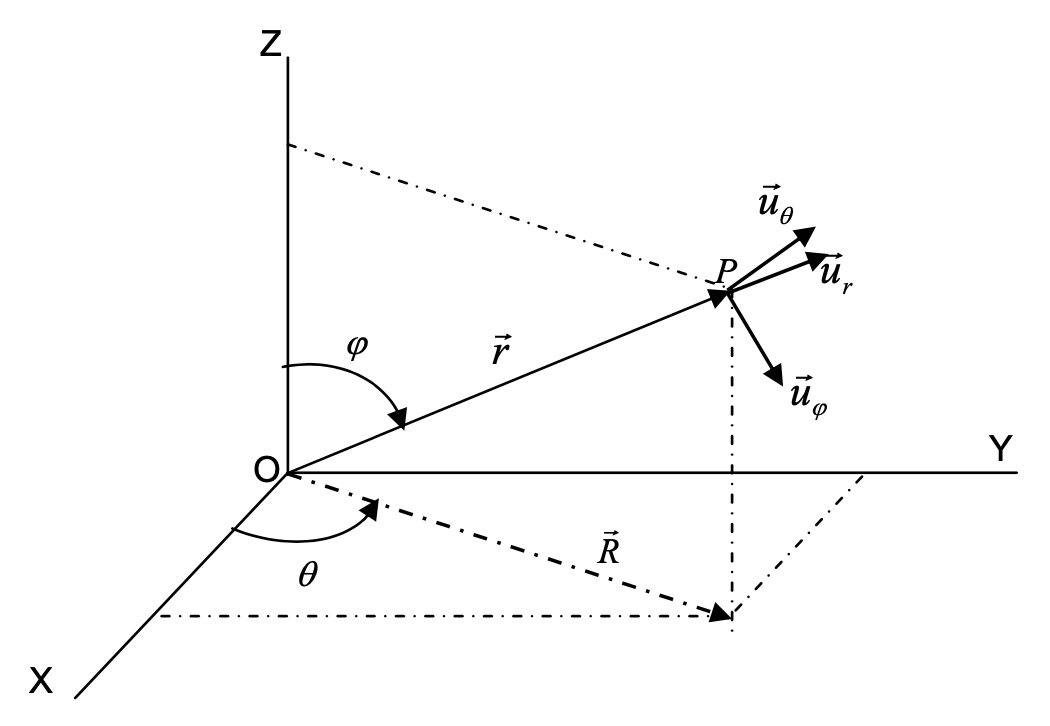
\includegraphics[width=.65\textwidth]{imagenes/apendices/APENDICESIM35.png}
\end{figure}


El vector director $\vec u_{r}$ está en la dirección $\overrightarrow{OP}=\vec r$.

l vector unitario $\vec u_{\phi}$ es perpendicular a $\vec u_{r}$ y su sentido es aquel en que $\phi$ crece.

l vector unitario $\vec u_{\theta}$ es perpendicular a los dos anteriores verificándose: $\vec u_{r} \times \vec u_{\phi} = \vec u_{\theta}$.

Un punto $P$ tiene un vector de posición que se encuentra en la dirección $OP$. En esféricas: $\vec r=r\; \vec u_r$ . No determina unívocamente su posición, solo indica que $P$ está a distancia $r$ del origen.


RELACIÓN DE LOS SISTEMAS DE COORDENADAS ESFÉRICAS Y RECTANGULARES.

\begin{figure}[H]
	\centering
	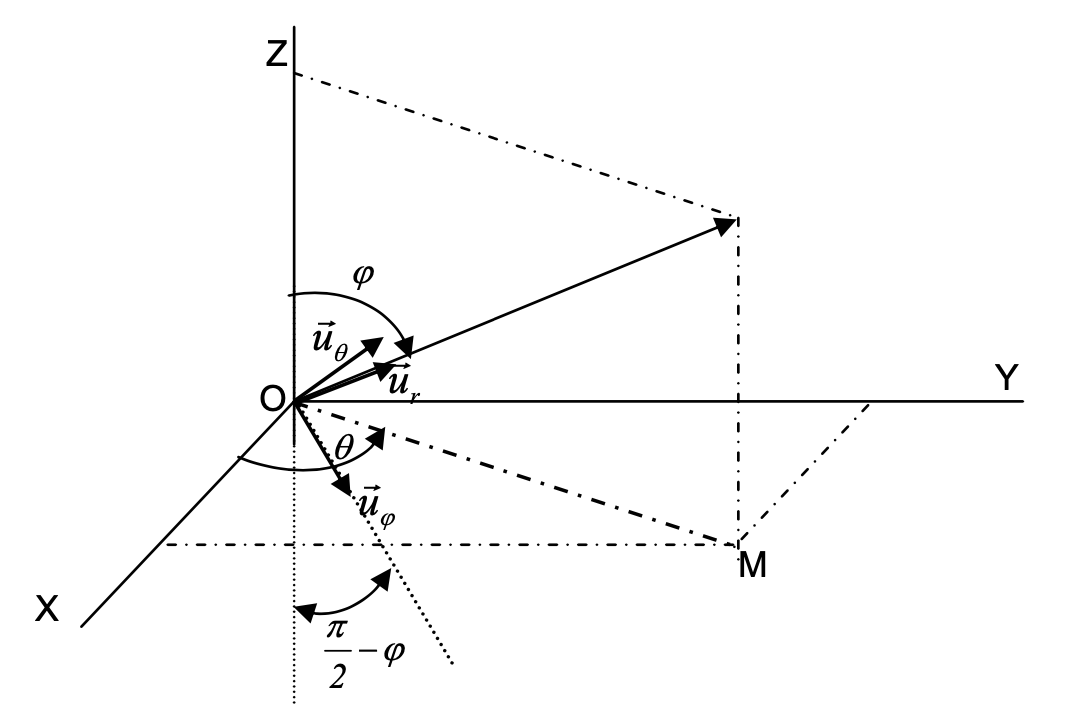
\includegraphics[width=.65\textwidth]{imagenes/apendices/APENDICESIM35b.png}
\end{figure}
Buscaremos las relaciones entre los vectores unitarios $\vec u_{r}$, $\vec u_{\theta}$, $\vec u_{phi}$ y los $\vec i$, $\vec j$, $\vec k$. Trasladamos los vectores unitarios al origen para facilitar el cálculo.

El vector $\vec u_{r}$ debe proyectarse previamente sobre el plano $XY$, dirección $OM$, antes de hacerlo sobre los ejes $X$ e $Y$. Esta proyección vale $\abs{\vec u_r} \sin \phi=1\; \sin \phi=\sin \phi$. Para proyectar $\vec {u_{\phi}}$  observamos que forma con el eje $Z$ un ángulo $(\frac \pi 2 - \phi)$ pero también debe ser proyectado antes sobre el plano $XY$ y después sobre los ejes.

Para proyectar $\vec {u_{\theta}}$ vemos que forma con el eje $X$, un ángulo $(\theta + \frac \pi 2)$.


$$\vec {u_r}=\sin \phi \cos \theta \;\vec i + \sin \phi \sin \theta \;\vec j + \cos \phi \; \vec k$$

$$\vec {u_{\phi}}=\sin (\frac \pi 2 -\phi) \cos \theta \; \vec i +\sin (\frac \pi 2 -\phi) \sin \theta \; \vec j - \cos (\frac \pi 2 - \phi)\; \vec k =$$ 
$$= \cos \phi \cos \theta \; \vec i + \cos \phi \sin \theta \; \vec j - \sin \phi \; \vec k$$

$$\vec {u_{\theta}}= \cos (\frac \pi 2 + \theta)\; \vec i + \sin (\frac \pi 2 + \theta)\; \vec j+0; \vec k = -\sin \theta \; \vec i + \cos \theta \vec j $$

\begin{ejem}
	Un punto tiene por coordenadas cartesianas $P(4,3,2)$, expresar su vector de posición en coordenadas esféricas.
\end{ejem}

$\abs{\vec r)}=\sqrt{4^2+3^2+2^2}=\sqrt{29};\qquad \vec r = r\; \vec u_r=29\; \vec u_r$

\begin{ejem}
	Expresar el vector $\vec v=-8\vec i+10 \vec j - 12 \vec k$ en coordenadas esféricas si su punto de aplicación está en $P(4,3,2)$.
\end{ejem}

Calculemos los vectores unitarios $\vec u_{r}$ $\vec u_{\theta}$, $\vec u_{\phi}$ en el punto $P(4,3,2)$. Obsérvese el vector $\vec R$ de la figura anterior a la anterior.

$\abs{\vec R}=\sqrt{4^2+3^2}=5; \quad \cos \theta =4/5=0.8;\quad \sin \theta=3/5=0.6;\quad \cos \phi=2/\sqrt{29};\quad \sin \phi=5/\sqrt{29}$

$$\vec u_r=\dfrac 5 {\sqrt{29}}\cdot 0.8 \; \vec i+\dfrac 5 {\sqrt{29}}\cdot 0.6 \; \vec j + \dfrac 2 {\sqrt{29}}\; \vec k = \dfrac  1{\sqrt{29}}\; (4\vec i+3\vec j+2\vec k)$$

$$ \vec {u_{\phi}}=\dfrac 2 {\sqrt{29}}\cdot 0.8 \;  \vec i + \dfrac 2 {\sqrt{29}}\cdot 0.6 \; \vec j - \dfrac 5 {\sqrt{29}}\; \vec k =
	\dfrac  1{\sqrt{29}}\; (1.6\vec i+1.2\vec j-5\vec k)$$

$$\vec {u_{\theta}}=-0.6\vec i+0.8 \vec j$$

Calcularemos las componentes del vector a$\vec v$ en las direcciones de los vectores unitarios $\vec u_{r}$ $\vec u_{\theta}$, $\vec u_{\phi}$ multiplicando escalarmente el vector por cada uno de estos unitarios.

$$ \vec v \cdot \vec {u_{r}}= (-8,10,-12)\cdot \frac 1 {\sqrt{29}} (4,3,2)=\frac {-26}{\sqrt{29}}$$ 

$$ \vec v \cdot \vec {u_{\phi}}= (-8,10,-12)\cdot \frac 1 {\sqrt{29}} (1.6,1.2,-5)=\frac {59.2}{\sqrt{29}}$$

$$ \vec v \cdot \vec {u_{\theta}}= (-8,10,-12)\cdot \frac 1 {\sqrt{29}} (-0.6,0.8,0)=12.8$$

Por lo que $\quad \vec {v_E}=\frac {-26}{\sqrt{29}}\; \vec {u_{r}}+ \frac {59.2}{\sqrt{29}}\; \vec {u_{\phi}}+ 12.8\; \vec {u_{\theta}}$.





\chapter{Introducción al cálculo vectorial}
\chaptermark{Cálculo Vectorial}

\section{Vector función de un escalar}

\begin{multicols}{2}
Un vector $\vec r$ es función de un escalar (número real) $t$ si lo es alguna de sus componentes:

$\boxed{ \; \vec r(t)=r_x(t) \ \vec i + r_y(t) \ \vec j + r_z(t) \ \vec k \; } \quad$
Tenemos una función de $\mathbb R \to \mathbb R^3\; : \; t \leadsto \vec {r(t)}$. 

Si tomamos todos los vectores con origen en $O$, sus extremos, para los distintos valores de $t$, dibujan una curva llamada `indicatriz' de ecuaciones paramétricas: $r_x=r_x(t); \; r_y=r_y(t); \; r_z=r_z(t)$. Si $t$ es el tiempo y $\vec r$ el vector de posición de una partícula, la `indicatriz' $ \vec r (t)$ será la `trayectoria'.

	\begin{figure}[H]
	\centering
	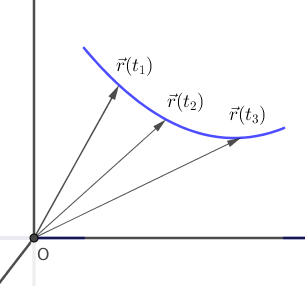
\includegraphics[width=0.4\textwidth]{imagenes/apendices/T10IM17.png}
	\end{figure}
\end{multicols}

\section{Derivada e integral de un vector}

\begin{multicols}{2}
	\begin{figure}[H]
	\centering
	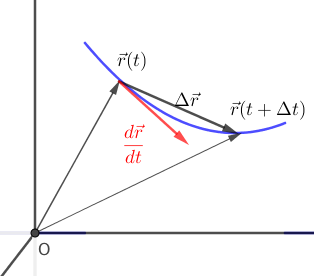
\includegraphics[width=0.35\textwidth]{imagenes/apendices/T10IM18.png}
	\end{figure}
Al pasar de $t$ a $t+ \Delta t \to \vec r (t)$ para a $\vec r (t+\Delta t)$ Si se incrementa la variable $t$ se incrementará el vector $\vec r$:

$\vec r (t) + \Delta \vec r = \vec r (t+\Delta t) = r_x (t+\Delta t) \vec i + r_y (t+\Delta t) \vec j + r_z (t+\Delta t) \vec k$

Despejando: $\Delta r =\vec r (t+\Delta t) - \vec r (t) = \Delta r_x \vec i +\Delta r_y \vec j +\Delta r_z \vec k \; $;  donde $\Delta r_x =  r_x (t+\Delta t) -  r_x (t) $ y análogamente para $\Delta r_y$ y $\Delta r_z$.
\end{multicols}

$\dfrac {\dd \vec r}{\dd t }= \underset{\Delta t \to 0}{lim}\; {\dfrac {\Delta r_x}{\Delta t}\;  \vec i} + \underset{\Delta t \to 0}{lim}\; {\dfrac {\Delta r_y}{\Delta t}\;  \vec j} + \underset{\Delta t \to 0}{lim}\; {\dfrac {\Delta r_z}{\Delta t}\;  \vec k}$

Es decir, la derivada de un vector respecto de un escalar es un vector cuyas componentes son las derivadas respecto del escalar de las respectivas componentes del vector a derivar.

\hspace{30mm}$\boxed{ \; \dfrac {\dd \vec r}{\dd t }= \overrightarrow {r'} = \dfrac {\dd r_x}{\dd t}\; \vec i + \dfrac {\dd r_y}{\dd t}\; \vec j + \dfrac {\dd r_z}{\dd t}\; \vec k\; }$

Por la interpretación geométrica de la derivada (\ref{IG-derivada}),el vector derivada es tangente a la curva indicatriz (trayectoria) (la dirección secante $\Delta \vec r$, con $\Delta t \to 0$ tiende a la dirección de la tangente $  \overrightarrow { r'} =\dfrac {\dd \vec r}{\dd t }\;$).

\vspace{4mm} \textbf {Reglas de derivación.} 

\begin{enumerate}[a) ]
\item Derivada de la suma de vectores: 
$\quad \dfrac {\dd {(\vec r + \vec s)}}{\dd t }$
$=\dfrac {\dd \vec r}{\dd t }+\dfrac {\dd \vec s}{\dd t }$

\item Derivada del producto por un escalar: $\quad \dfrac {\dd {(k\cdot \vec r)}}{\dd t }= k\cdot \dfrac {\dd \vec r}{\dd t }$
\item Derivada del producto escalar de dos vectores: $\quad \dfrac {\dd (\vec r \cdot \vec s)}{\dd t } = \dfrac {\dd \vec r}{\dd t }\cdot \vec s + \vec r \cdot \dfrac {\dd \vec s}{\dd t }$
\item Derivada del producto vectorial: $\dfrac {\dd (\vec r \times \vec s)}{\dd t }= \dfrac {\dd \vec r}{\dd t }\times \vec s + \vec r \times \dfrac {\dd \vec s}{\dd t }$	
\end{enumerate}

\underline{Propiedad} si $\vec r$ tiene módulo constante $\to$ es perpendicular a su vector derivada.

\begin{proof}\renewcommand{\qedsymbol}{$\diamond$}

Si $\vec r (t)$ tiene módulo cte. $\vec r (t) \cdot \vec r (t)= r^2 =cte.$. Derivado este producto escalar:

$\quad \dfrac {\dd (\vec r \cdot \vec r)}{\dd t }=2\vec r \cdot \dfrac {\dd \vec r}{\dd t}=0$, ya que $\dfrac {\dd \; cte}{\dd t}=0 \Rightarrow \; \boxed{\; |\vec r|=cte \leftrightarrow \displaystyle \vec r \; \bot \;  \dfrac {\dd \vec r}{\dd t }\;} $
\end{proof}

\vspace{4mm} \textbf{Integral de un vector}. Se define como la operación inversa a la derivada de un vector: la integral de un vector $\vec r(t)=r_x(t) \vec i + r_y(t) \vec j + r_z(t) \vec k$ es otro vector cuyas componentes son las integrales de las componentes del primero.

\hspace{20mm} $\boxed{ \; \displaystyle \int \vec r (t)\; \dd t = \vec i \; \int r_x (t)\; dd t + \vec j \; \int r_y (t)\; dd t+ \vec k \; \int r_z (t)\; dd t \; }$

\section{Campos escalares}

Una función escalar $\phi$ que toma valores en los puntos $x,y,z)$ del espacio se dice que es una función escalar de punto o, más simplemente, un `campo escalar' si:

A cada punto $P(x,y,z)$ del espacio, la función $\phi$ le asocia un número $\phi (x,y,z)\in \mathbb R$, es una aplicación de $\mathbb R^3$ en $\mathbb R$.

Ejemplos físicos de campos escalares son la temperatura (T), la presión (P), el potencial eléctrico (V), etc. 

El conjunto de todos los puntos del plano donde el campo $\phi$ toma un determinado valor $\phi_0$ forman una `superficie equiescalar', de ecuación: $\phi=\phi_0$.

\begin{multicols}{2}
Las superficies equiescalares pueden representar puntos que están a la misma temperatura (isotermas), a la misma presión (isóbaras), al mismo potencial eléctrico (superficies equipotenciales), etc.

\footnotesize{Si el campo esta definido en un plano las equiescalares serán líneas en vez de superficies. Como ejemplo, piénsese en las curvas de nivel de un mapa topográfico, $H(x,y)$ es la altura del punto $P(x,y)$ del mapa-2D}.

	\begin{figure}[H]
	\centering
	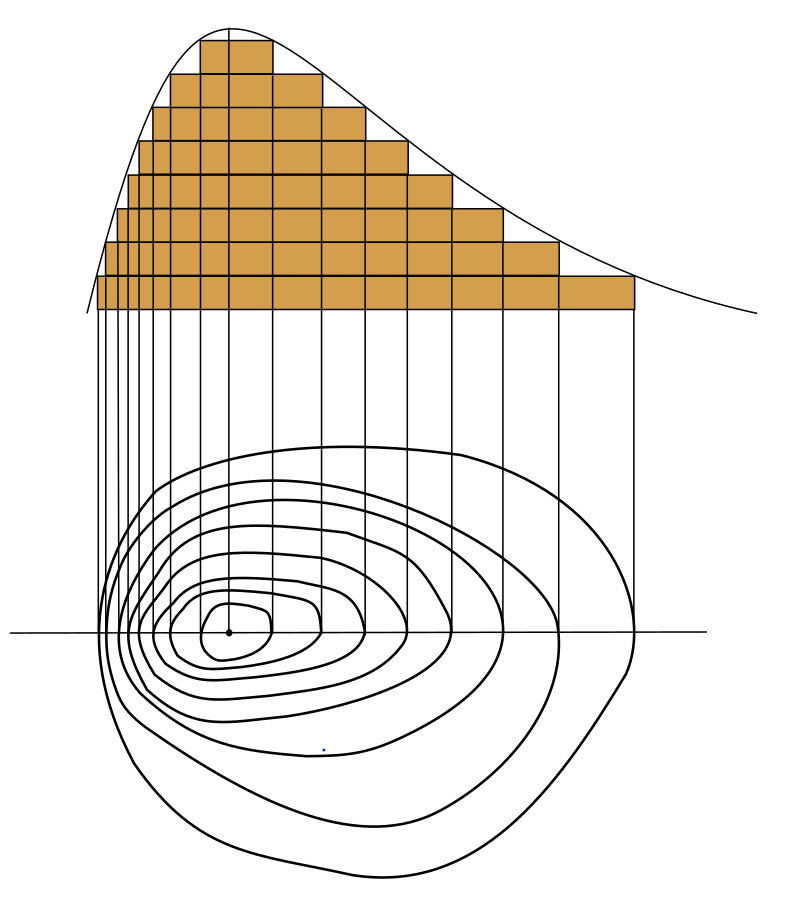
\includegraphics[width=0.25\textwidth]{imagenes/apendices/T10IM19.png}
	\end{figure}
\end{multicols}
\normalsize
En las funciones de una sola variable $y=f(x)$, la derivada (Leibniz) se define como el límite al que tiende el cociente $\Delta y / \Delta x$ cuando $\Delta x \to 0$, pero  un campo escalar $\phi (x,y,z)$ tendrá distintas derivadas ya que puede incrementarse una variable u otra, así, se define el crecimiento a lo largo del eje $OX$ como: $\Delta \phi_x =\phi (x+\Delta x, y, z)- \phi(x,y,z)$. Y su derivada, respecto de esta variable x, que se denota por $\dfrac{\partial \phi}{\partial x} = \underset {\Delta x \to 0}{lim}\;{\dfrac {\Delta \phi_x}{\Delta x}}= \eval {\dfrac {\dd \phi}{\dd x}}_{y,z=ctes.}\; \; $. Es decir, se trata de la derivada que resulta de suponer que $y$ y $z$ permanecen constantes y solo varía $x$. Análogamente se definen: $\dfrac{\partial \phi}{\partial y}=\eval {\dfrac {\dd \phi}{\dd y}}_{x,z=ctes.}\; $ y $\; \; \dfrac{\partial \phi}{\partial z}=\eval {\dfrac {\dd \phi}{\dd z}}_{x,y=ctes.}\; $. Esto es lo que se llama \underline{`derivadas parciales'}.

Las reglas de la derivación parcial son las mismas que para las funciones de una variable, solo hay que considerar que la variable sobre la que se deriva es realmente una variable y considerar al resto de variables como constantes.

Derivadas parciales: 

$\quad \boxed{\; \dfrac{\partial \phi}{\partial x}=\eval {\dfrac {\dd \phi}{\dd x}}_{y,z=ctes.} \quad \dfrac{\partial \phi}{\partial y}=\eval {\dfrac {\dd \phi}{\dd y}}_{z,x=ctes.} \quad \dfrac{\partial \phi}{\partial z}=\eval {\dfrac {\dd \phi}{\dd z}}_{x,y=ctes.} \;} $

\section{Campos Vectoriales}
\begin{multicols}{2}
	En matemáticas, un campo vectorial representa la distribución espacial de una magnitud vectorial. Es una expresión de cálculo vectorial que asocia un vector a cada punto en $\mathbb R^3$, de la forma $\vec E: \mathbb R^3 \to \mathbb R^3 \; : \vec E (x,y,z)= E_x \vec i + E_y \vec j + E_z \vec k$
	
	Los campos vectoriales se utilizan en física, por ejemplo, para representar la velocidad y la dirección de un fluido en el espacio, o la intensidad y la dirección de fuerzas como la gravitatoria o la fuerza electromagnética.
	
	\begin{figure}[H]
	\centering
	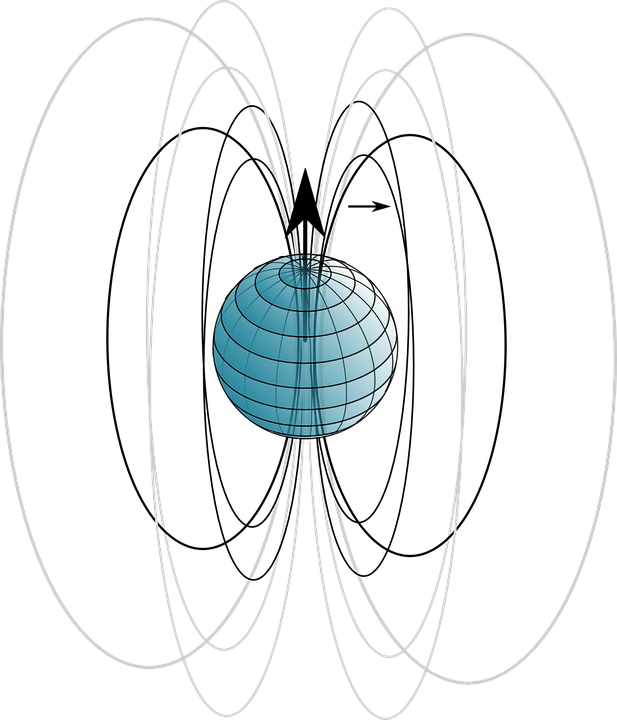
\includegraphics[width=0.35\textwidth]{imagenes/apendices/T10IM20.png}
	\end{figure}
\end{multicols}

\section{Gradiente de un campo escalar}

Sea $\phi (x,y,z)$ una función escalar, definida y derivable en cada uno de los puntos $(x.y.z)$ de una cierta región del espacio ($\phi$ es un campo escalar derivable), el `gradiente' de $\phi$, representado por $\overrightarrow {grad}\;  \phi\; $ o   $\; \overrightarrow{\nabla} \phi$ es un vector que se obtiene por la fórmula:

\vspace{4mm}\centerline{ $\boxed{ \; \overrightarrow {grad} \; \phi =  \overrightarrow {\nabla} \phi = \dfrac {\partial \phi}{\partial x}\; \vec i +  \dfrac {\partial \phi}{\partial y}\; \vec j +  \dfrac {\partial \phi}{\partial z}\; \vec k   \;} $}

Nótese que $\overrightarrow {grad} \; \phi $ define un `campo vectorial', es un vector que indica como varía $\phi$ en las proximidades de un punto, con el sentido del máximo crecimiento de la función.

Matemáticamente, la diferencial de una función $\phi (x.y.z)$ viene dada por:

\vspace{4mm}\centerline {$\boxed{ \; \dd \; \phi = \dfrac {\partial \phi}{\partial x}\; \dd x +  \dfrac {\partial \phi}{\partial y}\; \dd y + \dfrac {\partial \phi}{\partial z}\; \dd z \; }$}

\vspace{2mm} En notación de Leibniz, $\dd \phi$ representa la variación de $\phi$ entre dos puntos muy próximos: $x,y,z)\; $ y $\; (x+\dd x. y +\dd y, z +\dd z)$. Teniendo en cuenta la definición de gradiente:

\small{$\dd \; \phi = \dfrac {\partial \phi}{\partial x}\; \dd x +  \dfrac {\partial \phi}{\partial y}\; \dd y + \dfrac {\partial \phi}{\partial z}\; \dd z = \left( \dfrac {\partial \phi}{\partial x}\; \vec i + \dfrac {\partial \phi}{\partial y}\; \vec j + \dfrac {\partial \phi}{\partial z}\; \vec k     \right) \cdot (\dd x \; \vec i + \dd y \; \vec j + \dd z \; \vec k)$}\normalsize{.}

\begin{multicols}{2}
\vspace{3mm} Es decir:
 
$\boxed {\; \dd\; \phi = \overrightarrow {grad}\; \phi \cdot \dd \; \vec r = \overrightarrow { \nabla} \; \phi \cdot \dd \; \vec r \;} \quad$, 

donde $\dd \; \vec r = \dd x \; \vec i +\dd y \; \vec j + \dd z \; \vec k$, vector que une los puntos anteriormente señalados (desplazamiento infinitesimal). Esta ecuación determina la variación  $\dd \; \phi$ de la función escalar $\phi$ a lo largo de la dirección $\dd \; \vec r$. Des esta ecuación se deduce:

$\dd \; \phi = |\overrightarrow{\nabla}\; \phi |\cdot |\dd \vec r|\cdot \cos \theta$

	\begin{figure}[H]
	\centering
	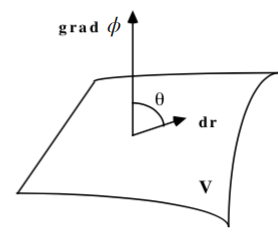
\includegraphics[width=0.4\textwidth]{imagenes/apendices/T10IM21.png}
	\end{figure}
\end{multicols}
deducimos que, para que exista una máxima variación del campo, para un valor fijo $|\dd \vec r|$, ha de ocurrir que 
$\cos \theta=1 \to \theta = 0\; $:  

\vspace{3mm}
\fbox{ \parbox{0.9\linewidth}{\emph{`El gradiente tiene la dirección de la máxima variación del campo y va en el sentido creciente de $\phi$'}}}
\vspace{3mm}

Las componentes del gradiente $\overrightarrow {\nabla} \; \phi$ en la dirección de un vector unitario $\overrightarrow {u_N}$ es igual al producto escalar $\overrightarrow {\nabla} \; \phi \cdot \overrightarrow {u_N} $ y se llama \textbf{derivada direccional} de $\phi$ en la dirección de $\overrightarrow {u_N}$ :

\centerline {$\boxed{\; \dfrac {\partial \phi}{\partial \overrightarrow {u_N}} = \overrightarrow {u_N} \cdot \overrightarrow {\nabla \phi}  \; }$}

\begin{multicols}{2}
Para una superficie $S$ determinada por la ecuación $f(x,y,z)=0$, el vector unitario normal en el punto $(x,y,z)$ viene dado por:

\hspace{15mm} $\overrightarrow {u_N}= \dfrac {\overrightarrow {\nabla f}}{|\overrightarrow {\nabla f}|}$

	\begin{figure}[H]
	\centering
	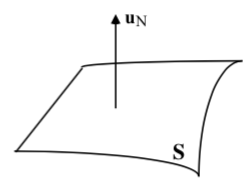
\includegraphics[width=0.3\textwidth]{imagenes/apendices/T10IM22.png}
	\end{figure}
\end{multicols}

La expresión: $ \overrightarrow {\nabla} \phi = \dfrac {\partial \phi}{\partial x}\; \vec i +  \dfrac {\partial \phi}{\partial y}\; \vec j +  \dfrac {\partial \phi}{\partial z}\; \vec k\;$, se puede obtener como el producto de un `operado vectorial' por un escalar , es decir:
$ \overrightarrow {\nabla} \phi = \left( \dfrac {\partial }{\partial x}\; \vec i +  \dfrac {\partial }{\partial y}\; \vec j +  \dfrac {\partial }{\partial z}\; \vec k \right) \cdot \phi\;$.
 El término dentro del paréntesis recibe el nombre de \textbf{`operado nabla'}:

\vspace{4mm}

\centerline{ $\boxed{ \; \overrightarrow {\nabla}=  \dfrac {\partial }{\partial x}\; \vec i +  \dfrac {\partial }{\partial y}\; \vec j +  \dfrac {\partial }{\partial z}\; \vec k \; }$}

\vspace{3mm}En resumen, el gradiente de una función escalar es un campo vectorial que tiene las siguientes propiedades:

 \begin{enumerate}

\item Sus componentes, en cada punto, son la razón de las variaciones de la función y de la coordenada a lo largo de las direcciones de los ejes en dicho punto. 

\item Su módulo, en cada punto, es el máximo valor de la variación de la función con la distancia. 

\item Su dirección es la de máxima variación. 

\item Su sentido es el de crecimiento de la función.

 \end{enumerate}
 
 El gradiente es, por tanto, un campo vectorial de punto deducido de un campo escalar de punto.
 
 \section{Divergencia de un campo vectorial}
 
 Sea $\vec E (x,y,z)=E_x \vec i + E_y \vec j + E_z \vec k\;$, una función vectorial definida y derivable en los puntos de una determinada región del espacio, $\vec E$ es un campo vectorial derivable.
 
 La divergencia de $\vec E$, representada por $div\; \vec E\;$ ó $\overrightarrow{\nabla}\cdot \vec E$, viene dada por la expresión:
 
 \vspace{4mm}\centerline{$\boxed{\; div\; \vec E = \overrightarrow{\nabla}\cdot \vec E = \dfrac {\partial E_x}{\partial x } + \dfrac {\partial E_y}{\partial y }+ \dfrac {\partial E_z}{\partial z } \; }$} 
 
 \vspace{3mm} que puede interpretarse como el `producto escalar' del operador $\overrightarrow{\nabla}$ por el campo vectorial $\vec E$, en ese orden y es, evidentemente, un escalar.
 
	La divergencia nos permite caracterizar aquellos puntos del campo vectorial en que éste, valga la expresión, `se crea o se destruye'; es decir, clasifica los manantiales o sumideros del campo. 

	Cuando $div \; \vec E = 0$ , no hay fuentes escalares del campo $\vec E$ , y se dice que el campo vectorial $\vec E$ es \textbf{\emph{solenoidal}}. 

	Si no existen `fuentes escalares' del campo éste no podrá `nacer` o `morir' en dichas fuentes, por lo cual las líneas del campo solenoidal son siempre cerradas. 

\section{Rotacional de un campo vectorial}

Sea $\vec E (x,y,z)=E_x \vec i + E_y \vec j + E_z \vec k\;$, un campo vectorial derivable, el rotacional de $\vec E$ , representado por $rot \; \vec E\; $ ó $\overrightarrow{\nabla} \times \vec E$ viene dado por la expresión:

\vspace{4mm} $rot \; \vec E = \overrightarrow{\nabla} \times \overrightarrow {E} = \left| \begin{matrix} \vec { i }  & \vec { j }  & \vec { k }  \\ \frac { \partial  }{ \partial x }  & \frac { \partial  }{ \partial y }  & \frac { \partial  }{ \partial z }  \\ \quad E_{ x } & E_{ y } & E_{ z } \end{matrix} \right| =$

$=\tiny{\left( \dfrac{\partial E_z}{\partial y} -\dfrac{\partial E_y}{\partial z} \right) \; \vec i + \left(\dfrac{\partial E_x}{\partial z} -\dfrac{\partial E_z}{\partial x} \right)\; \vec j+ \left(\dfrac{\partial E_y}{\partial x} -\dfrac{\partial E_x}{\partial y} \right)\; \vec k}$

\vspace{3mm}El rotacional de un vector puede entenderse como el `producto vectorial' del operador $\overrightarrow{\nabla}$ por el campo vectorial $\overrightarrow{E}$, en ese orden.

Cuando $\overrightarrow{\nabla} \times \overrightarrow {E}=\overrightarrow{0}$, se dice que el campo es \textbf{`ìrrotacional'} y nos permite decir que en campo $\overrightarrow {E}$ proviene de una función escalar $\phi$, en la forma:

$\overrightarrow{\nabla} \times \overrightarrow {E}=\overrightarrow{0} \longrightarrow \overrightarrow{E}-\overrightarrow{\nabla}\; \phi=-\overrightarrow{grad}\; \phi$

El valor del rotacional de un campo vectorial nos da las `fuentes vectoriales' del campo en cada punto. Si $\overrightarrow{\nabla} \times \overrightarrow {E}=\overrightarrow{0}$ para todos los puntos, entonces $\overrightarrow{E}$ no tiene fuentes vectoriales.

\section{Laplaciana de una función escalar}

Sea $\phi \; (x,y,z)$ un campo escalar definido u dos veces derivable en una determinada región del espacio. La laplaciana de $\phi$, representada por $\triangle\; \phi \;$ ó $\; \nabla^2 \; \phi$, lo determina la expresión:

\vspace{4mm}\centerline{$\boxed{\;\triangle\; \phi= \nabla^2 \; \phi =  \dfrac{\partial^2\; \phi}{\partial x^2}+\dfrac{\partial^2\; \phi}{\partial y^2}+\dfrac{\partial^2\; \phi}{\partial z^2} \;}$}

\vspace{3mm} La laplaciana es una función escalar.

Análogamente al `operador nabla', podemos definir el \textbf{`operador laplaciana'} como:


\vspace{4mm}\centerline{$\boxed {\;	\triangle = \nabla^2 = \dfrac {\partial^2}{\partial x^2}+ \dfrac {\partial^2}{\partial y^2}+\dfrac {\partial^2}{\partial z^2} \; }$}

Cuando el campo escalar $\phi$ tiene derivadas segundas continuas y se cumple $\triangle \; \phi = 0$, entonces se dice que el campo escalar $\phi$ es un `campo armónico'. La ecuación  $\triangle \; \phi = 0$ se llama \textbf{ecuación de Laplace}.

% *********************. Revisado el tema hasta aquí. 

\section{Ejercicios}

\begin{ejre}
Dado el campo vectorial $\overrightarrow A =x^2 \; \vec i + \sin y \; \vec j + zx \; \vec k$, encuentra: $\overrightarrow {\nabla} \cdot \overrightarrow A; \quad \overrightarrow \nabla \; (\overrightarrow {\nabla} \cdot \overrightarrow A); \quad \overrightarrow {\nabla} \times \overrightarrow A$	
\end{ejre}

\vspace{3mm}\begin{proof}\renewcommand{\qedsymbol}{$\diamond$}.	 

$\overrightarrow{\nabla}\cdot \vec A = \dfrac {\partial A_x}{\partial x } + \dfrac {\partial A_y}{\partial y }+ \dfrac {\partial A_z}{\partial z } = 3x+\cos y$	

$\overrightarrow \nabla \; (\overrightarrow {\nabla} \cdot \overrightarrow A)= \overrightarrow \nabla (3x+\cos y)= \dfrac {\partial (3x+\cos y)}{\partial x}\; \vec i + \dfrac {\partial (3x+\cos y)}{\partial y}\; \vec j +\dfrac {\partial (3x+\cos y)}{\partial z}\; \vec k = 3\; \vec i - \sin y \; \vec j$

$\overrightarrow {\nabla} \times \overrightarrow A = \left|
\begin{matrix}
\vec i & \vec j	& \vec k \\
\frac {\partial}{\partial x} & \frac {\partial}{\partial y} & \frac {\partial}{\partial z} \\
x^2 & \sin y & xz
\end{matrix}  \right|=\cdots =-z \vec i$
\end{proof}

\vspace{3mm}\begin{ejre}
$\overrightarrow A=2yz\; vec i -x^2y\; \vec j +xz^2\; \vec k\; $ y $\; \phi=2x^2yz^3\; $. Calcula: $\overrightarrow \nabla \; \phi; \quad \overrightarrow \nabla \cdot \overrightarrow A; \quad \overrightarrow \nabla \times \overrightarrow A; \quad \overrightarrow \nabla \cdot (\overrightarrow \nabla \; \phi); \quad \overrightarrow \nabla \; (\overrightarrow \nabla \cdot \overrightarrow A) $	
\end{ejre}

\vspace{3mm}\begin{proof}\renewcommand{\qedsymbol}{$\diamond$}.

$\overrightarrow \nabla \; \phi= \dfrac {\partial \phi}{\partial x}\; \vec i + \dfrac {\partial \phi}{\partial y}\; \vec j + \dfrac {\partial \phi}{\partial z}\; \vec k = 4xyz^3\; \vec i + 2x^2z^3\; \vec j + 6x^2yz^2\; \vec k$

$\overrightarrow \nabla \cdot \overrightarrow A=\dfrac {\partial A_x}{\partial x } + \dfrac {\partial A_y}{\partial y }+ \dfrac {\partial A_z}{\partial z }= -x^2+2xz$

$\overrightarrow \nabla \times \overrightarrow A== \left|
\begin{matrix}
\vec i & \vec j	& \vec k \\
\frac {\partial}{\partial x} & \frac {\partial}{\partial y} & \frac {\partial}{\partial z} \\
2yz & -x^2y & xz^2
\end{matrix}  \right|=\cdots =(2y-z^2) \vec j - (2xy+2z)\; \vec k$

$\overrightarrow \nabla \cdot (\overrightarrow \nabla \; \phi)= \overrightarrow \nabla \; ( 4xyz^3\; \vec i + 2x^2z^3\; \vec j + 6x^2yz^2\; \vec k)= \cdots = 4yz^3+12x^2yz$

$\overrightarrow \nabla \; (\overrightarrow \nabla \cdot \overrightarrow A)  =\overrightarrow \nabla (-x^2+2xz)=(-2x+2z)\, \vec i + 2x \; \vec k$

\end{proof}

\vspace{3mm}\begin{ejre}
Dado el campo escalar $\phi=(x,y,z)=2xz-3x^2+xy$, halla su derivada direccional en el pinto $(1,0,-3)$ según la dirección del vector unitario $\vec u = \widehat { u } =(-0.6,0,0.8)$ 
\end{ejre}

\vspace{3mm}\begin{proof}\renewcommand{\qedsymbol}{$\diamond$}.

La derivada direccional en la dirección y sentido de un vector unitario es la proyección del gradiente en esa dirección y sentido, es decir, su producto escalar (el de su gradiente) por dicho vector unitario.

$\dfrac {\partial \phi}{\partial \overrightarrow {u_N}} = \overrightarrow {u_N} \cdot \overrightarrow {\nabla \phi}; \quad \overrightarrow \nabla \; \phi = (-6x+y+2z) \vec i + x \vec j + 2x \vec k; \quad \eval {\overrightarrow \nabla \; \phi}|_{(1,0,-3}=(-12\vec i + \vec j + 3\vec k)$

$\eval {\dfrac { \partial \phi }{ \partial \overrightarrow {u_N} } }_{(1,0,-3)} = (-12,1,1)\cdot(-0.6,0,0.8)=8.8$
	
\end{proof}


\underline{Ejercicios propuestos}

\begin{enumerate}
\item Sea $\overrightarrow A = z \sin x \; \vec i + z \cos z \vec j + \sqrt{x^2+y^2}\; \vec k\; $, hallar:  	$\overrightarrow \nabla \; A; \quad   \overrightarrow {\nabla} \cdot \overrightarrow A; \quad \overrightarrow \nabla \; (\overrightarrow {\nabla} \cdot \overrightarrow A); \quad \overrightarrow {\nabla} \times \overrightarrow A; \quad \text { y } \quad \overrightarrow {\nabla} \times ( \overrightarrow \nabla \; A )\; $  donde $A =+\sqrt{\overrightarrow A \cdot \overrightarrow A}$, es el módulo de $\overrightarrow A$

\vspace{3mm} \textcolor{gris}{Sol: $A=r; \quad \overrightarrow \nabla \; A =\dfrac {x\vec i + y \vec j + z \vec k}{\sqrt{x^2+y^2+z^2}}=\vec r; \quad \overrightarrow \nabla \cdot \overrightarrow A= 0 $}

\textcolor{gris}{$\quad \overrightarrow \nabla (\overrightarrow \nabla \cdot \overrightarrow A)=\dfrac {2}{\sqrt{x^2+y^2+z^2}}=\dfrac 2 r ;\qquad \overrightarrow \nabla \times (\overrightarrow \nabla A ) =0$}


\textcolor{gris}{$ \quad \overrightarrow \nabla \times \overrightarrow A= \left( \dfrac {y}{\sqrt{x^2+y^2}-\cos z + z \sin z} \right)\; \vec i + \left (\sin z + z \cos z - \dfrac {x}{\sqrt{x^2+y^2}}  \right)\; \vec j$}

\item Dado el campo escalar $\; \phi=x^2yz+3x^2\; $ calcular su gradiente, la divergencia del gradiente y el rotacional del gradiente.

\vspace{3mm} \textcolor{gris}{Sol: $\overrightarrow \nabla \phi= (2xyz+6x)\vec i+x^2z\vec j+x^2y\vec k; \quad \overrightarrow \nabla \cdot(\overrightarrow \nabla \phi) = 2yz+6 ; \quad \overrightarrow \nabla \times (\overrightarrow \nabla \phi) =0$}
\end{enumerate}

\section{Los conceptos de campo} \label{concepto-campo}

\textcolor{gris}{ Reproduzco, por su interés, un artículo de}

\noindent \textcolor{gris}{ https://culturacientifica.com/2016/03/29/los-conceptos-campo/}
 
\noindent \textcolor{gris}{de EXPERIENTIA DOCET -ELECTROMAGNETISMO - (ARTÍCULO 8 DE 34) , de la Cátedra de Cultura Científica de la Universidad del País Vasco.}

\textcolor{gris}{ Experientia docet (blog) es el pseudónimo de César Tomé López,  licenciado en ciencias químicas (Universidad de Granada, 1989), . César Tomé López es divulgador científico y editor dE Mapping Ignorance.}

\vspace{4mm}

\textbf{Los conceptos de campo}

Gilbert describió la acción de la piedra imán diciendo que tenía una “esfera de influencia” alrededor de ella. Con esto quería decir que cualquier otro objeto magnético que entrase en esta “esfera” sería atraído por la piedra imán. Además, la intensidad de la fuerza atractiva sería mayor cuanto más cercano estuviese del imán. En términos actuales diríamos que la piedra imán está rodeada por un campo magnético. Experimentalmente podemos visualizar fácilmente un campo magnético o, más precisamente, la parte del mismo que intersecta el plano de una mesa, colocando sobre ésta un imán (idealmente con una forma regular) y esparciendo limaduras de hierro alrededor.

	\begin{figure}[H]
	\centering
	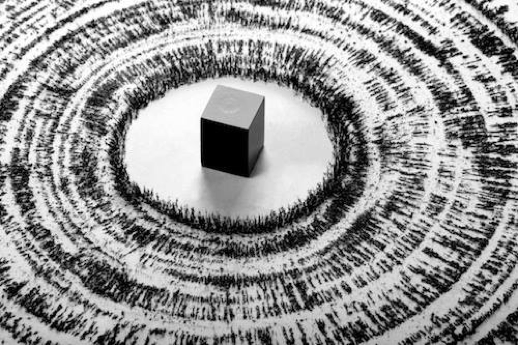
\includegraphics[width=.9\textwidth]{imagenes/apendices/ExperientiaDocet01.png}
	\end{figure}

La palabra “campo” se usa de maneras muy diversas y puede llevar a confusión, por lo que merece la pena que nos detengamos un momento en ella. Empezaremos por el uso común de la palabra para ir introduciendo después, de forma paulatina sus significados en física (efectivamente, sigue teniendo más de un sentido incluso en física). Este pequeño ejercicio nos permite de paso recordar que la mayoría de los términos usados en física son adaptaciones de palabras usadas en la vida ordinaria, pero a las que se dota de significados específicos. Otros ejemplos son velocidad, aceleración, fuerza, energía o trabajo. Comprender las diferencias entre el término físico y el común es fundamental para entender la física.

Uno de los usos comunes más frecuentes de la palabra campo (sobre todo en España) es “campo de juego” (en Iberoamérica quizás sea más frecuentemente “cancha”). Un campo de fútbol, por ejemplo, es un lugar donde dos equipos compiten según unas reglas que confinan la acción al área del campo. “Campo” en este caso significa región de interacción.

Otro uso habitual de la palabra campo se encuentra en el mundo de la geopolítica. En política internacional se habla de “esferas” o “campos” de influencia. Un campo de influencia política es también una región de interacción pero, a diferencia de un campo de juego, no posee una línea definida que marque sus límites. Unos países tienen más influencia que unos y menos que otros países. Por ello en el sentido político “campo” se refiere también a la cantidad de influencia, más en unos lugares y menos en otros. Además, en el caso político, el campo tiene una fuente, el país que ejerce la influencia.

Ya encontramos aquí similitudes con los conceptos de campo que se usan en física. Pero también con una diferencia importante. Para definir un campo en física tiene que ser posible asignar un valor numérico a la intensidad del campo en cada punto del campo. Esta parte del concepto de campo es más fácilmente entendible si consideramos dos situaciones de la vida cotidiana, primero en lenguaje ordinario y luego en términos físicos:

a) Voy andando por la acera, de noche, hacia una farola encendida. Veo que hay más luz conforme me acerco a ella.

b) Estoy quieto en una acera y oigo un coche que pasa de largo tocando la bocina de forma continua. Oigo que el sonido va aumentando de intensidad y luego disminuye.

	\begin{figure}[H]
	\centering
	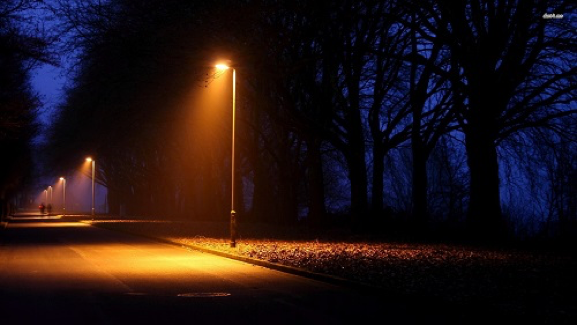
\includegraphics[width=.9\textwidth]{imagenes/apendices/ExperientiaDocet02.png}
	\end{figure}

Podemos describir estas dos situaciones usando campos:

a) La farola está rodeada por un campo de iluminación. Cuanto más cerca estoy de ella, más fuerte es el campo de iluminación que registra mi ojo o el medidor de intensidad de luz (fotómetro) que llevo conmigo. A cada punto del espacio alrededor de la farola puedo asignar un número que representa la intensidad del campo de iluminación en ese lugar.

b) La bocina del coche está rodeada por un campo de sonido. Yo estoy quieto en mi marco de referencia (la acera). Conforme el coche pasa a mi lado con él se mueve un patrón de valores de campo con la misma velocidad que el coche. Esto es, el campo de sonido es estable pero se mueve con la bocina. En cualquier caso yo puedo asignar un número a cada punto del campo para representar la intensidad del sonido. Al principio el sonido es apenas audible conforme la parte más débil del campo me alcanza. A partir de ahí comienza a subir la intensidad del campo y el sonido parece más fuerte. Finalmente, la intensidad disminuye al alejarse el campo de sonido y su fuente (la bocina).


Démonos cuenta de que en los campos que hemos considerado ambos están producidos por una sola fuente. En a) la fuente es una farola estacionaria y en b) es una bocina en movimiento. En ambos casos la intensidad del campo aumenta gradualmente conforme mi distancia a la fuente disminuye. Asociamos un valor numérico a cada punto del campo: estamos ante ejemplos de campos escalares sencillos. El concepto de dirección no aparece asociado al valor del campo en cada punto.

Entre los dos mapas que encuentras a continuación hay una diferencia significativa entre los campos representados en ambos. En el primero, en el que se representa la presión atmosférica y en el que las líneas (isobaras) unen puntos con igual valor de la presión, un solo número (una cantidad escalar) da el valor del campo en cada punto. Pero en el segundo, en el campo de la velocidad del viento, el valor del campo viene dado tanto por un valor numérico (llamado magnitud, representado por la escala de colores) y una dirección (representada por las flechas); la combinación de magnitud y dirección es lo que constituye un vector y por ello el campo de llama vectorial.
	
	
	\begin{multicols}{2}
	\begin{figure}[H]
	\centering
	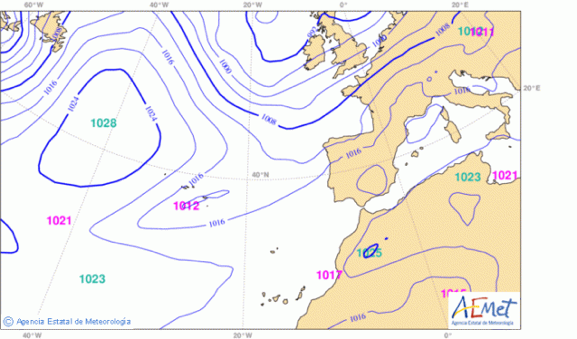
\includegraphics[width=0.5\textwidth]{imagenes/apendices/ExperientiaDocet03.png}
	\end{figure}
	Presión atmosférica
	\begin{figure}[H]
	\centering
	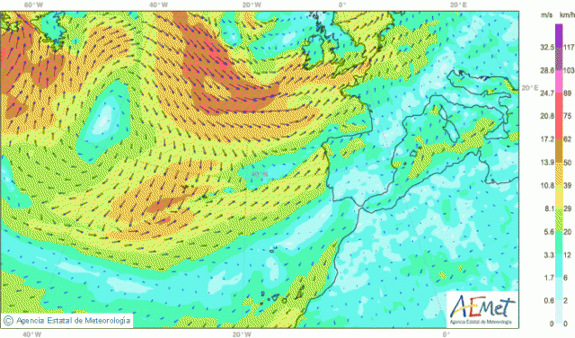
\includegraphics[width=0.5\textwidth]{imagenes/apendices/ExperientiaDocet04.png}
	\end{figure}
	Velocidad del viento	
	\end{multicols}





Finalmente, los físicos usan la palabra “campo” en tres sentidos adicionales a la definición de campo que hemos visto:

1) el valor del campo en un punto del espacio;

2) el conjunto de todos los valores en todos los puntos del espacio donde existe el campo;

3) la región del espacio en las que el campo toma valores distintos de cero.

Habitualmente, el contexto deja claro a cual de los conceptos de campo nos estamos refiriendo.

\vspace{4mm} \textcolor{gris}{Sobre el autor: \emph {César Tomé López es divulgador científico y editor de Mapping Ignorance.}}

\chapter{Introducción a las Ecuaciones Diferenciales}
\chaptermark{Introducción a las EDO}
\label{EDO}
\section{?`Qué son las ecuaciones diferenciales?}

Una ecuación diferencial es una ecuación matemática que relaciona una función con sus derivadas. En las matemáticas aplicadas, las funciones usualmente representan cantidades físicas, las derivadas representan sus razones de cambio, y la ecuación define la relación entre ellas. Como estas relaciones son muy comunes, las ecuaciones diferenciales juegan un rol primordial en diversas disciplinas, incluyendo la física, la ingeniería, la química, la economía, y la biología.

En las matemáticas puras, las ecuaciones diferenciales se estudian desde perspectivas diferentes, la mayoría concernientes al conjunto de las soluciones de las funciones que satisfacen la ecuación. Solo las ecuaciones diferenciales más simples se pueden resolver mediante fórmulas explícitas; sin embargo, se pueden determinar algunas propiedades de las soluciones de una cierta ecuación diferencial sin hallar su forma exacta. Si la solución exacta no puede hallarse, esta puede obtenerse numéricamente, mediante una aproximación usando ordenadores. 

Las ecuaciones diferenciales pueden dividirse en varios tipos. Aparte de describir las propiedades de la ecuación en si, las clases de las ecuaciones diferenciales pueden ayudar a buscar la elección de la aproximación a una solución. Es muy común que estas distinciones incluyan si la ecuación es: Ordinaria/Derivadas Parciales, Lineal/No lineal, y Homogénea/Inhomogénea. Esta lista es demasiado grande; hay muchas otras propiedades y subclases de ecuaciones diferenciales las cuales pueden ser muy útiles en contextos específicos.

Una ecuación diferencial ordinaria (EDO) es una ecuación que contiene una función de una variable independiente y sus derivadas. El término ``ordinaria'' se usa en contraste con la ecuación en derivadas parciales (`concepto que no hemos estudiado porque forma parte del cálculo con funciones de varias variables') la cual puede ser respecto a más de una variable independiente.

Las ecuaciones diferenciales lineales, las cuales tienen soluciones que pueden sumarse y ser multiplicadas por coeficientes, están bien definidas y comprendidas, y tienen soluciones exactas que pueden hallarse. En contraste, las EDOs cuyas soluciones no pueden sumarse son no lineales, y su solución es más intrincada, y muy pocas veces pueden hallarse en forma exacta de funciones elementales: las soluciones suelen obtenerse en forma de series o forma integral. Los métodos numéricos y gráficos para EDOs, pueden realizarse manualmente o mediante ordenadores, se pueden aproximar las soluciones de las EDOs y su resultado puede ser muy útil, muchas veces suficientes como para prescindir de la solución exacta y analítica.


\vspace{4mm}

APLICACIONES:

\vspace{3mm}

El estudio de ecuaciones diferenciales es un campo extenso en matemáticas puras y aplicadas, en física y en la ingeniería. Todas estas disciplinas se interesan en las propiedades de ecuaciones diferenciales de varios tipos. 

Las matemáticas puras se focalizan en la existencia y unicidad de las soluciones, mientras que las matemáticas aplicadas enfatizan la justificación rigurosa de los métodos de aproximación de las soluciones. Las ecuaciones diferenciales juegan un rol muy importante en el modelado virtual de cualquier proceso físico, técnico, o biológico, por ejemplo, tanto el movimiento celeste, como el diseño de un puente, o la interacción entre neuronas. Las ecuaciones diferenciales que se plantean para resolver problemas de la vida real, no necesariamente son resolubles directamente, es decir, sus soluciones no tienen una expresión en forma cerrada. Cuando sucede esto, las soluciones se pueden aproximar usando métodos numéricos.

Muchas leyes de la física y la química se formalizan con ecuaciones diferenciales. 

En biología y economía, las ecuaciones diferenciales se utilizan para el modelado del comportamiento de sistemas complejos. 

La teoría matemática de las ecuaciones diferenciales se desarrolló inicialmente con las ciencias donde las ecuaciones se originaban y donde se encontraban resultados para las aplicaciones. Sin embargo, algunas veces se originaban problemas diversos en campos científicos distintos, de los cuales resultaban ecuaciones diferenciales idénticas. Esto sucedía porque, detrás de la teoría matemática de las ecuaciones, puede verse un principio unificado detrás de los fenómenos. Como por ejemplo, si se considera la propagación de la luz y el sonido en la atmósfera, y de las ondas sobre la superficie de un estanque. Todos estos fenómenos pueden describirse con la misma ecuación en derivadas parciales de segundo orden, `la ecuación de onda', la cual nos permite pensar a la luz y al sonido como formas de onda, y en forma similar a las ondas en el agua. 

La conducción de calor, la teoría que fue desarrollada por Joseph Fourier, está gobernada por otra ecuación en derivadas parciales de segundo orden, `la ecuación de calor'. Resulta que muchos procesos de difusión, aunque aparentan ser diferentes, están descritos por la misma ecuación. 

\footnotesize{\textcolor{gris}{En física, las ecuaciones de campo de Einstein (conocidas como EFE, por Einstein Field Equations) son un conjunto de diez ecuaciones diferenciales de segundo grado en derivadas parciales de la tepría de la relatividad general de Albert Einstein que describen la interacción fundamental de la gravitación como resultado de que el espacio-tiempo está siendo curvado por la materia y ya energía. En el límite clásico no-relativista, esto es, a velocidades pequeñas  comparadas con la luz y campos gravitacionales relativamente débiles, las ecuaciones de campo de Einstein se reducen a la ecuación de Poisson para el campo gravitatorio, que es equivalente a la ley de gravitación de Newton}}\normalsize{.}

\rightline{\textcolor{gris}{Fuente: Wikipedia}}

\section{Ecuaciones diferenciales ordinarias}
	
	Sea $y=f(x)$, vamos a estudiar las ecuaciones donde intervienen la variable $x$, la función $y\;$ y alguna de sus derivadas $y';\; y''; \; y'''; \; \cdots$. Ejemplos de este tipo de ecuaciones son:
	$\quad xy'= y\; ; \qquad y''=y\; y'\; ; \qquad (y'')^2=\dfrac {x+y'}{1+x^2}$
	
\begin{defi}
Llamamos Ecuación Diferencial Ordinaria (EDO) a una ecuación el que intervengan la variable independiente $x$, una función $y(x)$ y una o varias derivadas de $y(x)$.	
\end{defi}

\begin{defi}
Llamamos `orden' de una EDO al orden de la mayor derivada que interviene en la ecuación. 
\end{defi}

Ejemplos: $\quad 2x+y\; y'=0 \text{ (orden 1) }\; ; \quad x^2 \dfrac {\dd^3 y}{\dd x^3}- \left( \dfrac {\dd y}{\dd x} \right)^4=1 \text{ (orden 3) }\; $

$ \dfrac {\dd^2 y}{\dd x^2}\; \cos x + \cos y =0 \text{ (orden 2) } $

Además,

\begin{defi}
Una EDO de orden `$n$' es `lineal' si se puede escribir en la forma:

\begin{equation}
	a_n(x)\; \dfrac {\dd^n y}{\dd x^n}+a_{n-1}(x)\; \dfrac {\dd^{n-1} y}{\dd x^{n-1}}+ \cdots + a_1(x)\;  \dfrac {\dd y}{\dd x}+a_0(x)\; y=b(x)
\end{equation}	
donde $a_i$ y $b$ solo dependen de $x$
\end{defi}

Ejemplos de EDO lineales:

$\sin x \; y''+y=e^x\; ; \quad \dfrac {1}{1+x^2}\; y'''+ (x^4-1)\; y=0\; ; \quad x\; \dfrac {\dd^4 y}{\dd x^4}+ x^2 \; \dfrac {\dd^2 y}{\dd x^2}+x^4\; y = x$

En cambio, no son EDO lineales:

$y\; y'=1;\qquad  \left( \dfrac{\dd y}{\dd x} \right)^2+y=0; \qquad \cos x\; \dfrac {\dd y}{\dd x}+\mathrm{ln} y=x\; \cos y$

\begin{defi}
Dada una EDO de orden $n$, llamamos `solución'	de la EDO a una función $y=f(x)$ definida en un intervalo $I$, de forma que cuando sustituimos $y=f(x)$ y sus derivadas en la EDO, ésta se verifica en todo $I$.
\end{defi}

\begin{ejem}
Consideremos la EDO $\quad y'+xy=x\; $	. Es fácil comprobar que la función $y=f(x)=1+e^{-{x^2}/2}\; $ es solución de esta EDO en todo $\mathbb R$, pero, la función $y=g(x)=1+k\cdot e^{-{x^2}/2}\; \; \text{ con } k\in \mathbb R \; $ también lo es.. Es decir, esta EDO tiene infinitas soluciones en $\mathbb R$.

Se recomienda al lector que compruebe lo dicho anteriormente.
\end{ejem}

\begin{ejem}
Para la EDO $\; y''+y=0\; $, las funciones $y=\sin x$ e $y=\cos x$ son soluciones en todo $\mathbb R$. Y, en general, dadas dos constantes $c_1, c_2 \in \mathbb R$, la función $y=c_1\; \sin x + c_2 \; \cos x$ también es solución en todo $\mathbb R$.

Se recomienda al lector que compruebe lo dicho anteriormente.
\end{ejem}

\begin{ejem}
Para la EDO $\; y'\; y^2=0 \;$	, la función $y=\dfrac 1 x$ es solución, pero en $\mathbb R^+$

Se recomienda al lector que compruebe lo dicho anteriormente.
\end{ejem}

Con los ejemplos vistos anteriormente, el conjunto de todas las soluciones de una EDO puede ser infinito. En ocasiones, nos interesa conocer solamente alguna de esas soluciones y no todas, por lo que se prefijan algunas condiciones previas a la solución buscada:

\begin{defi}{Problema de los Valores Iniciales.}

Dada una EDO de orden $n$ en un intervalo $I$ y un punto $x_0\in I$, llamamos `problema de los valores iniciales' (PVI, en lo que sigue) al problema de encontrar las soluciones de la EDO en $I$ y que además satisfagan las condiciones iniciales impuestas de antemano:

\begin{equation*}
	y(x_0)=c_0; \; y'(x_0)=c_1; \; y''(x_0)=c_2; \; \cdots ; \; y^{n-1}(x_0)=c_{n-1}
\end{equation*}

donde los $c_i$ son números prefijados.
\end{defi}

\begin{ejem}.

--- El problema PVI $\; \begin{cases} 2y\; y'=e^x \\ y(0)=0 \end{cases}\; $. Tiene como solución la función $y=e^{x/2}\; $. Puede comprobarse que es la única solución que admite el problema.

--- El problema PVI $\; \begin{cases} 2y\; y'=e^x \\ y(0)=-1 \end{cases}\; $, tiene como única solución $y=-e^{x/2}$. Compruébese.

--- La EDO de segundo orden $y''-y=x$ tiene por soluciones todas las funciones de la forma $y=-x+c_1 e^x+c_2 e^{-x} \; \forall c_1, c_2 \in \mathbb R \; $, Así, el PVI dado por $\; \begin{cases} 2y \; y'=e^x \\ y(1)=0; \; y'(1)=0 \end{cases}\; $, tiene como íunica solución $y=-x+e^{x-1}$. Compruébese.

Aunque en los ejemplos anteriores los PVI tienen solución única, pude haber problemas PVI en que hayan más de una solución.
\end{ejem}

\section{Modelos matemáticos de problemas de ciencia}

En muchas ocasiones es deseable describir en términos matemáticos el comportamiento de algunos sistemas o fenómenos de la vida real, tanto de tipo físico, químico, sociológico, económico... La descripción matemática de un sistema de fenómenos se llama `modelo matemático' y se construye con ciertos objetivos, como el de entender que ocurrirá en el futuro o que ocurrió en el pasado. Por ejemplo, podemos desear entender los mecanismos de cierto ecosistema al estudiar el crecimiento de la población animal en ese sistema, o podemos desear datar fósiles y analizar el decaimiento de una sustancia radiactiva ya sea en el fósil o en el estrato en que éste fue descubierto. 

Para la realización de un modelo matemático sobre un sistema, primero hay que identificar todas las variables que ocasionan que el sistema cambie y posteriormente establecer de qué manera estas variables afectan al sistema. Es claro que cuantas más variables que afectan al sistema se añadan mejor resolución tendrá el modelo que se obtenga. Sin embargo, el modelo será cada vez más complejo cuantas más variables entren en juego. Por ello, a veces un modelo de baja resolución (es decir, con pocas variables) es suficiente para determinar de forma aproximada la solución de nuestro problema. 

A continuación estudiaremos algunos modelos matemáticos clásicos en diferentes áreas de las Ciencias.

\subsection{Dinámica poblacional}

Dinámica poblacional. 
El economista Thomas Malthus hizo uno de los primeros intentos para modelar el crecimiento de una población. Así, supuso que la razón de la población en un cierto tiempo $t$ es proporcional a la población total en ese tiempo. Es decir, si llamamos $P(t)$ a la población en el tiempo $t$ entonces se obtiene que 

\begin{equation*}
	\dfrac {\dd P}{\dd t}=k\; P\; ,
\end{equation*}

donde $k$ es una constante que depende de la población estudiada.

Aunque este modelo es de baja resolución, aún así sigue siendo útil para el estudio de algunas poblaciones a tiempo corto, como, por ejemplo, poblaciones de cultivos de bacterias. 


\subsection{Decaimiento radiactivo}    


El núcleo de algunos átomos están formados por combinaciones de protones y neutrones inestables, es decir, los átomos se desintegran o se convierten en átomos de otras sustancias. En estos casos se dice que los núcleos son radiactivos. Por ejemplo, el radio $^{ 226 }{ Ra }$, intensamente radiactivo, se transforma en gas radón $^{ 222 }{ Rn }$.
 
Para modelar el fenómeno de decaimiento radiactivo, dada una cantidad $A(t)$ de una sustancia en el tiempo $t$, se supone que la razón con la que los núcleos se desintegran es proporcional a la cantidad existente, esto es, 
\begin{equation*}
	\dfrac {\dd A}{\dd t}= k\; A\; ,
\end{equation*}

con $k$ una constante que depende de la sustancia estudiada. 

\subsection{Ley de calentamiento-enfriamiento de Newton}
  
La ley empírica de enfriamiento/calentamiento de Newton establece que la rapidez con la que cambia la temperatura de un cuerpo es proporcional a la diferencia entre la temperatura del cuerpo y la del medio que lo rodea (la temperatura ambiente). 
 
Si denotamos por $T(t)$ a la temperatura del cuerpo en el tiempo $t$ y $T_a$ a la temperatura del ambiente, entonces, la ley de enfriamiento/calentamiento de Newton determina que 
  
  \begin{equation*}
  	\dfrac {\dd T}{\dd t}= k\; \left( T(t)-T_a \right)\; ,
  \end{equation*}
  
donde k es la constante de proporcionalidad. 

\subsection{Reacciones químicas} 
  
En algunas reacciones químicas la rapidez con la que las moléculas de una sustancia $A$ se descomponen es proporcional a la cantidad de sustancia que queda sin reaccionar. Así, si llamamos $c(t)$ a la cantidad de la sustancia $A$ en el tiempo $t$ entonces 
  
 \begin{equation*}
 	\dfrac {\dd c(t)}{\dd t}= k\;( A\;- \; c(t)) ,
 \end{equation*} 
    
donde k es una constante (dependiente de la sustancia A).
  
   
Un ejemplo de este tipo, llamada reacción de primer orden, está dada por la conversión del cloruro de terbutilo $(CH_3)_3CCl$ en alcohol t-butílico $(CH_3)_3COH$: 
   
\begin{equation*}
	(CH_3)_3CCl \; + \; NaOH \longrightarrow (CH_3)_3COH\; + \; NaCl
\end{equation*}
   
   Solo la concentración de cloruro de terbutilo controla la rapidez de la reacción. 
   
   Sin embargo, en la reacción 
   
   \begin{equation*}
   	CH_3Cl + NaOH \longrightarrow  CH_3OH + NaCl \; ,
   \end{equation*}
   
la razón con la que avanza la reacción es proporcional al producto de las concentraciones de cloruro de metilo $CH_3Cl$ y de hidróxido de sodio $NaCl$ que quedan. 
   
   Para describir en general una reacción de este tipo, conocida como reacción de segundo orden, supongamos que se combina una molécula de una sustancia $A$ con una molécula de una sustancia $B$ para formar una molécula de una sustancia $C$ (más otras sustancias). Si $c(t)$ denota la cantidad de la sustancia $C$ que se ha formado en el tiempo $t$ y si $a_0,\; b_0$ son, respectivamente, las cantidades de las sustancias $A$ y $B$ en el momento inicial $t = 0$, entonces las cantidades de $A$ y $B$ en tiempo $t$ son $a_0- c(t)$ y $b_0- c(t)$, respectivamente. Así, la razón de formación de $C$ está dada por 
   
\begin{equation*}
	\frac {\dd c}{\dd t}=k(a_0-c)(b_0-c)\; ,
\end{equation*} 
   
donde k es una constante de proporcionalidad. 

\subsection{Mezclas} 
   
   Supongamos que en un tanque mezclador tenemos $300$ litros de agua con sal. Por otro lado, un grifo de entrada introduce $3$ litros de agua por minuto, que tiene una concentración de $2$ gramos por litro. La solución bien mezclada sale del tanque con la misma rapidez de $3$ litros por minuto. 
   
De esta manera, si denotamos por $A(t)$ a la cantidad de sal en el tanque al tiempo $t$, entonces la razón con la que $A(t)$ cambia viene dada por 
   
   \begin{equation*}
   	\dfrac {\dd A}{\dd t}= \text{ (razón de entrada de sal)-(razón de salida de sal)}\; .
   \end{equation*}
   
La razón de entrada de sal es de $(2g/l) \cdot (3l/min) = 6g/min$. Por otra parte, ya que la cantidad de agua en el tanque es constantemente de $300$ litros, la 
razón de salida de sal es de $\displaystyle \left(\dfrac {A(t)}{300}\; g/l \right) \cdot \left( 3 \; l/min \right)=\dfrac {A(t)}{100}\; g/min$
   
De esta manera, 
   
   \begin{equation*}
   	\dfrac {\dd A}{\dd t}=6-\dfrac {A}{100}
   \end{equation*}
   

\subsection{Cuerpos en caída y resistencia del aire}
   
Aunque a un cuerpo en caída en el vacío solo le afecta la fuerza de la gravedad, en general, cuando no se encuentra en el vacío, el aire ejerce una resistencia al movimiento en la caída de un cuerpo. 
   
   Así , el peso del cuerpo es una fuerza que actúa en la dirección de  caída, mientras que la resistencia del aire actúa en dirección opuesta. La fuerza $F_r$ dada por la resistencia del aire se denomina amortiguamiento viscoso y es proporcional a la velocidad del cuerpo, esto es, $F_r = k\; v$, donde $k$ es una constante que depende del cuerpo y $v$ su velocidad. 
   
	La segunda ley del movimiento de Newton determina que la suma de las fuerzas ejercidas sobre el cuerpo es igual a su masa $m$ por su aceleración $a=\dfrac {\dd v}{\dd t}$, es decir, 
   
\begin{equation*}
	m\; \dfrac {\dd v}{\dd t} = m\; g - k\; v\;;
\end{equation*} 
   
donde $g$ es la aceleración de la gravedad.
   
   O equivalentemente, si denotamos por $s(t)$ al espacio recorrido en el tiempo t entonces 
   
 \begin{equation*}
 	m\; \dfrac {\dd^2 s}{\dd t^2} = m\; g - k\; \dfrac {\dd s}{\dd t}
 \end{equation*} 
 
 \vspace{3mm}
 
 \emph{La resolución de estas ecuaciones diferenciales son, en primera aproximación, una solución a los problemas planteados.}
 \section{EDOs de primer orden}
 
 En esta sección estudiaremos algunas EDO de primer orden. Hay que tener en cuenta que, en ocasiones, la solución $y(x)$ del problema aparecerá en forma implícita y en algunos casos no será posible despejarla de la ecuación:

$y^2+2xy+x^2=0;\to y\;  \text { despejable }; \quad
y+\cos y=x^3-1; \to y\;  \text { no despejable }$


\subsection{EDOs separables}

\begin{defi}
Decimos que una EDO de primer orden es `separable' o que tiene variables separables se se puede escribir en la forma: $\displaystyle \quad  \boxed{\;  g(y)\; \dfrac {\dd y}{\dd x}=h(x)\;} $
\end{defi}

Por ejemplo, la EDO $y'=e^{x-2y}\; \cos x$ es `separable', pues se puede escribir como $e^{2y}\; \dfrac {\dd y}{\dd x}=e^x\; \cos x\; $;  en cambio, la EDO $y'=y^2-\sin x\; $ no es `separable'.

\vspace{2mm}

\emph{Observación:} Una ecuación del tipo $y'=f(y)\cdot g(x)$ se puede escribir como una EDO separable de la forma $\dfrac 1 {f(y)}\; \dfrac {\dd y}{\dd x} = g(x)\;$ , pero en este caso hay que tener en cuenta que $f(y)\neq 0$, además, los números $c\; / \; f(c)=0$ cumplen que la función constante $y(x)=c$ es una solución de la EDO pues al sustituir en la ecuación original la verifican.

Así, p.e., la EDO $\; y'=(1-y^2)\; x^2\; $ es separable, se puede escribir en la forma $\frac 1 {1-y^2}\; \frac {\dd y}{\dd x}= x^2\;$. Hay que tener en cuenta, en esta ocasión, que las funciones $y(x)=1$ e $y(x)=-1$ son dos soluciones de la EDO original (soluciones de $1-y^2=0$).

\begin{teor}{Resolución EDOs separables.}

	Dada la EDO: $\displaystyle \quad  g(y)\; \dfrac {\dd y}{\dd x}=h(x)\; $ basta con escribirla en la forma: $\; g(y)\; \dd y = h(x)\; \dd x$ e integrar a ambos lados de la igualdad:
	\begin{equation*}
		\boxed{\; \int g(y)\; \dd y = \int h(x)\; \dd x\; }
	\end{equation*}
	Y así se obtienen todas las soluciones de la EDO de forma implícita.
\end{teor}

\begin{ejem}
$y^2\; y'=x-2 \to y^2\; \dd y = (x-2) \; \dd x \to y^3=x^2-2x+\mathcal C \leftrightarrow y=\sqrt[3]{x^2-2x+\mathcal C}$	
\end{ejem}

\begin{ejem}
$y'=\dfrac {y}{1+x^2} \to \dfrac {\dd y}{y} = \dfrac {\dd x}{1 + x^2} \to \mathrm{ln}|y|=\arctan x + \mathcal C\; ; \quad  \forall \mathcal C_0 \in \mathbb R; $.
Recuérdese que la solución $y=0$ también es solución de la EDO (*).

Tomando exponenciales: $y=\mathcal C_0\; e^{\arctan x}$, con $ 	\mathcal C_0=e^{\mathcal C} \;$. Esta forma general, tomando $\mathcal C_0=0$ incluye la solución $y(x)=0$ (*). 
\end{ejem}

\begin{ejem}
Sea el PVI $\begin{cases} e^{x+y} \cdot  y'= x \\ y(0)=0 \end{cases}\quad$. 

La ecuación puede escribirse como $e^y\dd y=xe^{-x}\dd x$, integrando por partes (\emph{hágase}) se obtiene: $e^y=-(1+x)e^{-x}+\mathcal C$.

Imponiendo la condición inicial $y(0)=0 \to 1=-1+\mathcal C \to \mathcal C=2$. Con lo que la solución del PVI es: $e^y=-(1+x)e^{-x}+2 \leftrightarrow y=\left(2-(1+x)e^{-x}\right)$.
	
\end{ejem}

\begin{ejem}
Sea el PVI $\begin{cases}  y'= -2x y^2 \\ y(3)=1/10 \end{cases}\quad \to \dfrac {\dd y}{y^2}=-2x \dd x $. Nótese que, al dividir por $y^2$, podría ocurrir que $y(x)=0$ que es solución de la EDO pero no del PVI, no cumple la condición inicial $y(3)=1/10$-

Integrado: $-\dfrac 1 y = -x^2+\mathcal C \to y=\dfrac {1}{x^2 - \mathcal C}$. Imponiendo la condición inicial se obtiene (\emph{hágase}) $\; y=\dfrac {1}{x^2 + 1}$
\end{ejem}

\subsection{EDOs lineales de primer orden}

Son otras EDOs, de primer orden que se pueden resolver de forma sencilla

\begin{defi}
Una EDO es de primer orden `lineal' si se puede escribir en la forma:

\begin{equation*}
	\boxed{\; a_1(x)\; y' +a_0(x)\; y = b(x)\;} 
\end{equation*}	
Con $a_1, a_0, b$ funciones que solo dependen de $x$.
\end{defi}

Poe ejemplo: $y'+x^2y=e^x \cos x\; $, ó \; $e^x y' +y =x^3$, son EDO lineales de primer orden. Sin embargo, $y'+y^2=\sen x\; $ ó $\; yy'+xy=e^x$ no lo son.

\begin{defi}
Decimos que una EDO lineal de primer orden es \textbf{homogénea} si:

 $\quad b(x)=0\qquad$, es decir, $\quad  a_1(x)\; y' +a_0(x)\; y = 0$	
\end{defi}

Ejemplos de EDO lineales de primer orden homogéneas son. $\; \sin (x)\; y' + \cos(x)\; y = 0\; $ ó $\; e^x\; y'+y=0\; $ ó $\; (x^2+1) \; y'+x\; y=0$.

\begin{teor}{Resolución EDOs lineales de primer orden.}

Para resolver la ecuación $\; a_1(x)\; y' +a_0(x)\; y = b(x)\; $, primero hay que resolver la ecuación homogénea asociada $a_1(x)\; y' +a_0(x)\; y = 0\; $. Esta última EDO es `separable' y puede resolverse como lo explicado en el apartado anterior. la solución de la EDO homogénea es de la forma $\; y(x)=\mathcal{C}_0\; y_1(x)\;$ para una cierta constante $\mathcal{C}_0$.

Si $b(x) \neq 0$, las soluciones de la ecuación  $\; a_1(x)\; y' +a_0(x)\; y = b(x)\; $ serán de la forma $y(x)=u(x)\; y_1(x)$, para una cierta función $u(x)$ a determinar. Es decir, se sustituirá la constante $\mathcal{C}_o$ dada en la EDO lineal homogénea por una función $u(x)$.

Para determinar esta  $u(x)$ se sustituirá la solución $y(x)=u(x)\; y_1(x)$ sobre la ecuación original $\; a_1(x)\; y' +a_0(x)\; y = b(x)\; $ y de ahí obtendremos una ecuación de donde podremos despejar $u'(x)$. Finalmente, por integración de esta $u'(x)$ obtendremos la  $u(x)$ y, por tanto, las soluciones de la EDO lineal de primer orden. 	
\end{teor}


\begin{ejem}
	La EDO $(1+x^2)\; y' + x\; y = 0$ el lineal, de primer orden y homogénea, por lo que la podemos resolver como `separable':
	
	$\dfrac {\dd y}{y }=-\dfrac {x}{1+x^2}$. Siempre que $y \neq 0$. De hecho, $y=0$ es solución del problema. Integrando:
	
	$\mathrm{ln} |y|=-\frac 1 2 \; \mathrm{ln} (1+x^2)+\mathcal{C} \leftrightarrow y=\dfrac {\mathcal{C}_0}{\sqrt{1+x^2}}\;$. para cualquier $\mathcal{C}_0$ real; solución que incluye a $y=0$, tomando $\mathcal{C}_0=0$
\end{ejem}



\begin{ejem}
Considera la EDO lineal de primero orden: 

$\; \arctan(y)\; y'- \dfrac {2}{1+x^2}\; y=\arctan^3 (x)\; $	

Primero resolveremos la EDO homogénea: $\; \arctan(y)\; y'- \dfrac {2}{1+x^2} \; y=0\; $

La podemos escribir, para $y\neq 0$ como separable:

$\dfrac {\dd y}{y }= \dfrac {2\; \dd x} {\arctan (x) \cdot (1+x^2)}  \; $ Se trata de una integral potencial inmediata (\emph{resuélvase}). 

El resultado es: $\; y=\mathcal {C}_0 \; \arctan^2 (x)$ 

Pare encontrar las locuciones de la EDO original, $\; \arctan(y)\; y'- \dfrac {2}{1+x^2}\; y=\arctan^3 (x)\; $, consideraremos funciones de la forma: $\; y=u(x) \cdot  \arctan^2 (x)\; $ y sustituimos en la ecuación original:

$\arctan^3 (x)= \arctan (x) \cdot \left( u(x)\cdot \arctan^2 (x) \right)' \; - \; \dfrac {2}{1+x^2} \cdot \left( u(x) \cdot  \arctan^2 (x) \right) = u'\; \arctan^3 (x)$

Tenemos que $u'(x)=1 \to u(x)=x+\mathcal C$, así, la solución de la EDO inicialmente propuesta es: 
$\; y=(x+	\mathcal C)\; \arctan^2 (x)$

\end{ejem}

\begin{ejem}

Considera el PVI: $\begin{cases} xy'-x^2y=e^{x^2/2} \\ y(1)=-1 \end{cases}$

Empezamos por resolver la EDO homogénea asociada: $\; xy'-x^2y=0\; $, que puede ser escrita (separable): $\dfrac {\dd y}{y}=x\; \dd x$. Para $y\neq 0$, integrando obtenemos (\emph{compruébese}) : $\; y=\mathcal{C}_0\; e^{x^2/2} \; $ 

Las soluciones de la EDO $\; xy'-x^2y=e^{x^2/2} \; $ serán de la forma: $y=u(x)\; e^{x^2/2}\; $. Determinaremos $u(x)$ sustituyendo la solución en la ecuación inicial:

$e^{x^2/2}=xy'-x^2y=x\; \left( u(x)\; e^{x^2/2} \right)' - x^2\, \left( u(x)\; e^{-x^2/2} \right) =x\; y'(x)\; e^{x^2/2}\; $, de donde $u'(x)= \dfrac {1} {x} \to u=\mathrm{ln}|x|+\mathcal C\; $. Así, todas las soluciones de la EDO serán: 

$\; y=\left(c+\mathrm{ln}|x| \right)\; e^{x^2/2}\;$ . Imponiendo, ahora, la condición inicial $y(1)=-1 \to c=-\dfrac {1}{\sqrt{e}}\;$ (\emph{compruébese}), con lo que la solución al PVI planteado es: 
$y=\left( \dfrac {1}{\sqrt{e}} + \mathrm{ln} x  \right) \; e^{x^2/2}$

\end{ejem}

\begin{ejem}

PVI: $\begin{cases} xy'-y=\dfrac {x^2}{1+x^2} \\ y(-1)=\pi/4 \end{cases}\; $, resolvemos primero la EDO homogénea:

$xy'-y=0 \to \dfrac{\dd y}{y}= \dfrac {\dd x }{x}\; $, para $y\neq 0\; $, (\emph{compruébese}), $y=\mathcal{C}_0\; x$ 

Las soluciones de la EDO $\; xy'-y=\dfrac {x^2}{1+x^2} \; $ serán de la forma:$\; y= u(x) \cdot  x \; $. sustituyendo:
$\dfrac {x^2}{1+x^2}= xy'-y=x\; \left( u(x) \cdots x \right)' - u(x) \cdot x =u'(x) \cdot x^2$

Por tanto, $\; u'(x)=\dfrac {1}{1+x^2}  \to u(x)=\arctan x + \mathcal C$

Las soluciones de la EDO lineal de primer orden es $\; y=\left( \mathcal C + \arctan x \right)\; x\; $ . Imponiendo la condición inicial del PVI, $y(-1)=\pi/4\; $ (\emph{hágase}), la solución del problema es: $\;y=x\; \arctan x \; $

\end{ejem}



\section{EDOs lineales de segundo orden}

\begin{defi}
Las EDO lineales de segundo orden son de la forma:

\begin{equation*}
  \boxed{ \; a_2\; y'' + a_1	\; y' + a_0 y= b(x) \; }
\end{equation*}
	Con $a_0\neq 0, \; b_0$ constantes reales y $h(x)$ una función de $x$
\end{defi}

\begin{teor}{Resolución EDOs lineales de segundo orden homogéneas.}

Las soluciones de una EDO de segundo orden lineal homogénea $\; a_2\; y'' + a_1	\; y' + a_0 y= b(x) \;$ son de la forma: $y(x)=\mathcal{C}_1\; y_1(x)+\mathcal{C}_2\; y_2(x)\;$. Las constantes $\mathcal{C}_1, \mathcal{C}_2$ y las funciones $y_1(x), y_2(x)$ se encuentra del siguiente modo:

Considera la ecuación de segundo grado \; $a_2\;  m^2 + a_1 \; m + a_0=0\; $ y tomamos las soluciones \; $m_1,\;  m_2\; $ de esta ecuación. Ahora distinguimos tres casos según sean estos valores:

\begin{enumerate}

\item  Si $\; m_1,\; m_2\; $	son dos números reales distintos ($\Delta=a_1^4-4a_a\cdot a_0>0$), entonces:

\begin{equation*}
	y_1(x)=e^{m_1\; x} \; ;  \qquad  \qquad y_2(x)=e^{m_2\; x}
\end{equation*}

\item Si $m_1=m_2\; $,  ($\Delta=0$), entonces:

\begin{equation*}
	y_1(x)=e^{m_1\; x} \; ;  \qquad  \qquad y_2(x)=x\; e^{m_1\; x}
\end{equation*}

\item Si las raíces son complejas conjugadas ($\Delta<0$), 
$\; m_1=\alpha + \beta \; i\; $ ; $\; m_1=\alpha - \beta \; i\; $ ($\alpha, \beta in \mathbb R$), entonces:

\begin{equation*}
	y_1=e^{\alpha\; x}\; \cos (\beta\; x) \; ;  \qquad  \qquad y_2=e^{\alpha\; x}\; \sin (\beta\; x)
\end{equation*}
\end{enumerate}
\end{teor}

\vspace{4mm}

\begin{ejem}
$y''-3y'+2y=0 \to m^2-3m+2=0 \to m_1=1 \; \wedge m_2=2\; $

Entonces, las soluciones de la EDO son: $\; y=\mathcal{C}_1\; e^x +\mathcal{C}_2\; e^{2x}\; , \quad \forall \mathcal{C}_1,\mathcal{C}_2 \in \mathbb R$  	
\end{ejem}

\begin{ejem}
La EDO $\; 4y''-4y'+y=0\; $ tiene por ecuación de segundo grado asociada $\; 4m^2-4m+1=0 \to m_1=m-_2=\frac 1 2 \; $.

Las soluciones de la EDO son: $\; y=\mathcal{C}_1\; e^{x/2} + \mathcal{C}_2\;x\; e^{x/2} \; , \quad \forall \mathcal{C}_1,\mathcal{C}_2 \in \mathbb R$
\end{ejem}



\begin{ejem}
$y''-4y'+13y=0 \to m^2-4m+13=0 \to 	m=2\pm 3\; i$

\noindent Soluciones de la EDO: $\ \; y= \mathcal{C}_1\; e^{2x} \cos (3x) + \mathcal{C}_2\; e^{2x} \sin  (3x) \; , \ \forall \mathcal{C}_1,\mathcal{C}_2 \in \mathbb R$
\end{ejem}



\begin{ejem}
PVI: $\; \begin{cases} y''-4y'+5y=0 \\ y(0)=3; \; y'(0)=1 \end{cases}$

Primero resolvemos la EDO, cuyo polinomio asociado es: $,^2-4m+5=0 \to m=2\pm  i$. Por ello, las soluciones de la EDO son:
$\; y= \mathcal{C}_1\; e^{2x} \cos (x) + \mathcal{C}_2\; e^{2x} \sin  (x) \; , \quad \forall \mathcal{C}_1,\mathcal{C}_2 \in \mathbb R$

Imponiendo las condiciones iniciales: $\quad y(0)=3; \; y'(0)=1 \; $ (\emph{hágase}), obtenemos la solución de PVI: $\quad y=e^{2x}\; (3\cos x-5\sin x)$
	
\end{ejem}

\vspace{3mm}

Para la EDO lineal de segundo orden lineal tiene la forma: $\; a_2\; y'' + a_1	\; y' + a_0 y= b(x)\; $, con $\; b(x) \neq  0\; $, la solución se obtiene de otro modo, como se explica en el siguiente teorema:


\begin{teor}{Resolución EDOs lineales de segundo orden generales.}

Dada $\; a_2\; y'' + a_1	\; y' + a_0 y= b(x)\; $, primero se resuelve la ecuación homogénea asociada, es de decir: $\; a_2\; y'' + a_1	\; y' + a_0 y= 0 \; $ y se encuentran sus soluciones, del tipo: $\; y=\mathcal{C}_1\; y_1(x) +\mathcal{C}_2\; y_2(x)\; , \quad \forall \mathcal{C}_1,\mathcal{C}_2 \in \mathbb R\; $ e $y_1(x),\; y_2(x)\; $ funciones de $x$.  que se obtienen como se ha explicado en el teorema anterior.

Las soluciones de la EDO general serán de la forma $\; y= u_1(x)\; y_1(x) \; + \; u_2(x)\; y_2(x)\; $, donde las funciones $u_i$ se encuentran al resolver el sistema:

\begin{equation*}
	\begin{cases}
	u'_1(x)\; u_1(x) + u'(2)\; y_2(x)=0 \\
	u'_1(x)\; y'_1(x) + u'_2(x)\; y'_2(x)= \dfrac {b(x)}{a_2}	
	\end{cases}	
\end{equation*}

Las derivadas $u'_i(x)$ se han de integrar y ya se obtiene la solución.	
\end{teor}

\vspace{4mm}


\begin{ejem}
$y''+y'-2y=3e^x \to $ Primero resolvemos la EDO homogénea: 

$y''+y'-2y=0 \to m^2+m-2=0 \to m_1=1 \; \wedge \; m_2=-2 $

Las soluciones de la EDO homogénea son:  $y=\mathcal{C}_1 e^x + \mathcal{C}_2 e^{-2x}$. Montemos el sistema:

$\begin{cases}
u'_1(x)\; e^x + u'_2(x)\; e^{-2x}=0 \\
u'_1(x)\; e^x - 2x \; u'_2(x)\; e^{-2x}= 3e^x	
\end{cases} \to $ Resolviendo el sistema (\emph{hágase}):

$u'_1(x)=1 \to u_1(x)=x + \mathcal{C}_1 ; \quad u'_2(x)=-e^{3x} \to u_2(x)=-\frac 1 3 e^{3x}+\mathcal{C}_2$. La soluciones de la EDO gral. son (\emph{hágase}):

\hspace{20mm} $y=\left( x+\mathcal{C}_1 \right)\; e^x + \left( -\frac 1 3 e^{3x} + \mathcal{C}_2 \right) \; e^{-2x}=(*)= (x+\mathcal{D}_1) \; e^x + \mathcal{C}_2\; e^{-2x}$, 

con $\mathcal{D}_1, \; \mathcal{C}_2$ constantes reales por determinar.

\rightline{\textcolor{gris}{(*) $e^{3x} \cdot e^{-2x}=e^x$}}
	
\end{ejem}



\begin{ejem}
$9y''+6y'+y=\sin x \to : \; $ EDO homogénea: $9y''+6y'+y=0 \to :\; $  Polinomio asociado: $9m^2+6m+1=0 \to m_1=m_2=-\frac 1 3 \to : \; $ Soluciones de la EDO homogénea: $y=\mathcal{C}_1 \; e^{-x/3} + \mathcal{C}_2 \; x \; e^{-x/3} \to :\; $	Sistema de ecuaciones para determinar las $u_i$:

$\begin{cases}
u'_1(x)\; e^{-x/3} + u'_2(x) \; x \; e^{-x/3} = 0 \\
-\frac 1 3 \; u'_1(x)\; e^{-x/3} - \frac 1 3 \; (x-3)\;  u'_2(x)\ e^{-x/3} = \frac {\sin x}{9} 	
\end{cases}$

Resolviendo el sistema anterior (\emph{hágase}), se obtiene:

$\quad u_1(x)=-\frac 1 9 \; x \; e^{-x/3}\; \sin x ; \quad  u'_2(x)= \frac 1 9 \; e^{x/3} \; \sin x\; $, ahora, integrando (\emph{hágase}), se obtienen las funciones $u_i$:

$u_1(x)=\mathcal{C}_1+\frac 1 {150}\;  e^{-x/3} \; \left( 3(5x-3)\cos x -(5x+12)\sin x \right)\;$

$u_2(x)=\mathcal{C}_2 - \frac 1 {30} \; e^{-x/3}\; (3\cos x-\sin x)$

Con lo que las soluciones de la EDO gral son:

\hspace{30mm} $y=\mathcal{C}_1 \; e^{-x/3}+\mathcal{C}_2 \; x \; e^{-x/3}- \frac 1 {50} \; (3\cos x + 4 \sin x)$

\end{ejem}


\begin{ejem}
	$y''+2y'+2y=e^{-x} \to y''+2y'+2y=0 \to m^2+2m+2=0 \to m=-2 \pm i$

Soluciones EDO homogénea: $y=\mathcal{C}_1 e^{-x} \cos x + \mathcal{C}_2 e^{-x} \sin x \; \to \; $ Sistema:

$\begin{cases}
u'_1(x)e^{-x} \cos x + u'_2(x) e^{-x} \sin x = 0 \\
-u'_1(x) e^{-x} (\cos x + \sin x ) + u'_2(x) e^{-x} (\cos x - \sin x )=e^{-x}	
\end{cases}$

Soluciones e integrales: $u'_1(x)=-\sin x \to u_1(x)=\mathcal{C}_1 + \cos x ; \quad u'_2(x)=\cos x \to u_2(x)=\mathcal{C}_2 +\sin x$ Y la solución de la EDO lineal de segundo orden lineal es:

\hspace{30mm} $y=e^{-x}\cdot \left( 1+ \mathcal{C}_1 \; \cos x + \mathcal{C}_2 \; \sin x \right)$ 


\end{ejem}

\begin{ejem}
	PVI: $\; \begin{cases} y''-6y'+9y=2e^3x \\ y(0)=1; \; y'(0)=-2 \end{cases}$

Resolvemos primero la EDO homogénea: $y''-6y'+9y=0 \to m^2-6m+9=0 \to m_1=m_2=3$

Soluciones de la EDO homogénea: $y=\mathcal{C}_1 \; e^{3x} + \mathcal{C}_2\; x \; e^{3x}$

Sistema: $\; \begin{cases}
 u'_1(x)\; e^{3x} + u'_2(x) x e^{3x} =0 \\
 3u'_1(x) e^{3x}+(3x+1) u'_2(x) e^{3x}=2 e^{3x}	
 \end{cases} 	$
 
 $\to \begin{cases}
 u'_1(x)= -2x \to u_1(x)=-x^2 + \mathcal{C}_1 \\
 u'_2(x)=2 \to u_2(x)=2x+\mathcal{C}_2	
 \end{cases}$
 
 Con todo ello, la solución de la EDO gral. es:  $\; y=e^{3x}\; (x^2+\mathcal{C}_2\; x + \mathcal{C}_1)$
 
 Finalmente, imponiendo las condiciones iniciales $y(0)=1; \; y'(0)=-2$, se obtiene, como solución de PVI:
 
 \hspace{30mm} $y=e^{3x}\; (x^2-5x+1)$
 
 \rightline{\textcolor{gris}{\emph{háganse todos los pasos que faltan.}}}

\end{ejem}



\textit{La redacción de este capítulo es copia `casi' textual de los apuntes de catedrático de apuntes del catedrático J.A. Gálvez, del departamento de geometría y topología de la universidad de Granada. Muchas gracias por compartir tu saber.}

\section{Aplicaciones de las ecuaciones diferenciales}

\rightline{\textit{Fuente: wikipedia}}

\vspace{3mm}

\textcolor{gris}{
El estudio de ecuaciones diferenciales es un campo extenso en matemáticas puras y  aplicadas, en física y en la ingeniería. Las ecuaciones diferenciales juegan un rol muy importante en el modelado virtual de cualquier proceso físico, técnico, o biológico, por ejemplo, tanto el movimiento celeste, como el diseño de un puente, o la interacción entre neuronas. Las ecuaciones diferenciales que se plantean para resolver problemas de la vida real, no necesariamente son resolubles directamente, es decir, sus soluciones no tienen una expresión en forma cerrada. Cuando sucede esto, las soluciones se pueden aproximar usando métodos numéricos.}

\textcolor{gris}{Muchas leyes de la física y la química se formalizan con ecuaciones diferenciales. En biología y economía, las ecuaciones diferenciales se utilizan para el modelado del comportamiento de sistemas complejos. La teoría matemática de las ecuaciones diferenciales se desarrolló inicialmente con las ciencias donde las ecuaciones se originaban y donde se encontraban resultados para las aplicaciones. Sin embargo, algunas veces se originaban problemas diversos en campos científicos distintos, de los cuales resultaban ecuaciones diferenciales idénticas. Esto sucedía porque, detrás de la teoría matemática de las ecuaciones, puede verse un principio unificado detrás de los fenómenos. Como por ejemplo, si se considera la propagación de la luz y el sonido en la atmósfera, y de las ondas sobre la superficie de un estanque. Todos estos fenómenos pueden describirse con la misma ecuación en derivadas parciales de segundo orden, la ecuación de onda, la cual nos permite pensar a la luz y al sonido como formas de onda, y en forma similar a las ondas en el agua. La conducción de calor, la teoría que fue desarrollada por Joseph Fourier, está gobernada por otra ecuación en derivadas parciales de segundo orden, la ecuación de calor. Resulta que muchos procesos de difusión, aunque aparentan ser diferentes, están descritos por la misma ecuación. La ecuación de Black-Scholes en las finanzas, está por ejemplo, relacionada con la ecuación del calor.}

\textcolor{gris}{\textbf{Física}}

\textcolor{gris}{•	Ecuaciones de Euler-Lagrange en mecánica clásica.}

\textcolor{gris}{•	Ecuaciones de Hamilton en mecánica clásica.}

\textcolor{gris}{•	Radiactividad en física nuclear.}

\textcolor{gris}{•	Ley de enfriamiento de Newton en termodinámica.}

\textcolor{gris}{•	Ecuación de onda.}

\textcolor{gris}{•	Ecuación de calor en termodinámica.}

\textcolor{gris}{•	Ecuación de Laplace, que define las funciones armónicas.}

\textcolor{gris}{•	Ecuación de Poisson.}

\textcolor{gris}{•	Ecuación geodésica.}

\textcolor{gris}{•	Ecuaciones de Navier-Stokes en fluidodinámica.}

\textcolor{gris}{•	Ecuación de difusión en procesos estocásticos.}

\textcolor{gris}{•	Ecuación de convección-difusión en fluidodinámica.}

\textcolor{gris}{•	Ecuaciones de Cauchy-Riemann en análisis complejo.}

\textcolor{gris}{•	Ecuación de Poisson-Boltzmann en dinámica molecular.}

\textcolor{gris}{•	Ecuaciones de Saint-Venant.}

\textcolor{gris}{•	Ecuación diferencial universal.}

\textcolor{gris}{•	Ecuaciones de Lorenz cuyas soluciones exhiben un flujo caótico.}

\textcolor{gris}{\textbf{Mecánica clásica.}}


\textcolor{gris}{Siempre que se conozca la fuerza actuante sobre una partícula, la Segunda ley de Newton es suficiente para describir el movimiento de una partícula. Una vez que están disponibles las relaciones independientes para cada fuerza que actúa sobre una partícula, se pueden sustituir en la segunda ley de Newton para obtener una ecuación diferencial ordinaria, la cual se denomina ecuación de movimiento}.

\textcolor{gris}{\textbf{Electrodinámica.}}

\textcolor{gris}{Las ecuaciones de Maxwell son un conjunto de ecuaciones en derivadas parciales que, junto con la ley de la fuerza de Lorentz , forman los fundamentos de la electrodinámica clásica, óptica clásica, y la teoría de los circuitos eléctricos. Estos campos se volvieron fundamentales en las tecnologías eléctricas, electrónicas y de comunicaciones. Las ecuaciones de Maxwell describen cómo los campos eléctrico y magnético se generan alterando uno y otro por cargas y corrientes eléctricas. Estas ecuaciones deben su nombre al físicomatemático escocés James Clerk Maxwell, quien publicó sus trabajos sobre estas ecuaciones entre 1861 y 1862.}

\textcolor{gris}{\textbf{Relatividad general.}}

\textcolor{gris}{Representación de la curvatura dada por la ecuación de campo de Einstein sobre el plano de la eclíptica de una estrella esférica: Dicha ecuación relaciona la presencia de materia con la curvatura adquirida por el espacio-tiempo.}

\textcolor{gris}{Las ecuaciones de campo de Einstein (conocidas también como ``ecuaciones de Einstein'') son un conjunto de diez ecuaciones en derivadas parciales de la teoría de la relatividad general donde se describe la interacción fundamental de la gravitación como un resultado de que el espacio-tiempo es curvado por la materia y la energía.}
 
\textcolor{gris}{Publicado por primera vez por Einstein en 1915 como una ecuación tensorial, las ecuaciones equiparan una curvatura espacio-tiempo local (expresada por el tensor de Einstein) con la energía y momentum local dentro del espacio-tiempo (expresado por el tensor de energía-impulso).}

\textcolor{gris}{\textbf{Mecánica cuántica.}}

\textcolor{gris}{En la mecánica cuántica, el análogo a la ley de Newton es la Ecuación de Schrödinger (una ecuación en derivadas parciales) para un sistema cuantificado (usualmente átomos, moléculas, y partículas subatómicas que pueden estar libres, ligadas, o localizadas). No es una ecuación algebraica simple, pero es, en general, una ecuación en derivadas parciales y lineal, que describe la evolución en el tiempo de una función de onda (también llamada una "función de estado").}

\textcolor{gris}{\textbf{Biología.}}
 
\textcolor{gris}{•	Ecuación de Verhulst – para el crecimiento de población biológica.}
 
\textcolor{gris}{•	Modelo de von Bertalanffy – para el crecimiento individual biológico.}
 
\textcolor{gris}{•	Dinámica de replicación – en teoría biológica.}
 
\textcolor{gris}{•	Modelo de Hodgkin y Huxley – potenciales de acción neuronal.}
	
\textcolor{gris}{\textbf{Ecuaciones predador-presa.}}

\textcolor{gris}{Las ecuaciones Lotka–Volterra, también conocidas como las ecuaciones predador-presa, son un par de ecuaciones diferenciales no lineales de primer orden frecuentemente utilizadas para describir la dinámica de sistemas biológicos en los cuales interactúan dos especies, una el predador, y la otra, la presa. }

\textcolor{gris}{\textbf{etc...}}



\chapter*{}
	